\documentclass[11pt,letterpaper]{article}

% ============================================================================
% PACKAGES
% ============================================================================
\usepackage[utf8]{inputenc}
\usepackage[T1]{fontenc}
\usepackage{helvet}
\renewcommand{\familydefault}{\sfdefault}
\usepackage[margin=0.85in, headheight=32pt, headsep=18pt, footskip=30pt]{geometry}
\usepackage{graphicx}
\usepackage[table]{xcolor}
\usepackage{tikz}
\usepackage{pgfplots}
\pgfplotsset{compat=1.18}
\usepackage{tcolorbox}
\usepackage{booktabs}
\usepackage{enumitem}
\usepackage{xurl}
\usepackage{hyperref}
\usepackage{fancyhdr}
\usepackage{titlesec}
\usepackage{titletoc}
\usepackage{upquote}
\usepackage{amsmath,amssymb}
\usepackage{array}
\usepackage{longtable}
\usepackage{colortbl}
\usepackage{pifont}
\usepackage{setspace}
\usepackage{parskip}
\usepackage{caption}
\usepackage{tabularx}
\usepackage{float}
\usepackage{needspace}
\usepackage{flafter}

% Ragged-right paragraph columns
\newcolumntype{L}[1]{>{\raggedright\arraybackslash}p{#1}}
\newcolumntype{Y}{>{\raggedright\arraybackslash}X}

\usetikzlibrary{shapes.geometric, shapes.misc, arrows.meta, positioning, calc, decorations.pathreplacing, backgrounds, fit}

% ============================================================================
% COLOR DEFINITIONS - shared hardware-series palette (deep indigo + amber)
% ============================================================================
\definecolor{deepindigo}{HTML}{1A237E}
\definecolor{indigo}{HTML}{3949AB}
\definecolor{nightink}{HTML}{0D1333}
\definecolor{honeyamber}{HTML}{FFA000}
\definecolor{darkamber}{HTML}{C77700}
\definecolor{alertcrimson}{HTML}{C62828}
\definecolor{ledgerviolet}{HTML}{6A1B9A}
\definecolor{sensorteal}{HTML}{00838F}
\definecolor{proxygray}{HTML}{78909C}
\definecolor{campaignred}{HTML}{AD1457}
\definecolor{paleindigo}{HTML}{EEF0FA}
\definecolor{medgray}{HTML}{BDC3C7}
\definecolor{softslate}{HTML}{5C6480}
\definecolor{textdark}{HTML}{1C2233}

\color{textdark}

\captionsetup[figure]{font={small,sf}, labelfont={bf,color=deepindigo}, skip=8pt, margin=0.5cm}

% ============================================================================
% HYPERREF SETUP
% ============================================================================
\hypersetup{
  colorlinks=true,
  linkcolor=deepindigo,
  citecolor=darkamber,
  urlcolor=indigo,
  pdftitle={Recurrent Depth Signatures: Detecting Looped and Recurrent-Depth Language Models from the Outside (v1.0, October 2026)},
  pdfauthor={Hardware Systems Documentation},
  pdfsubject={Measurement methods for distinguishing recurrent-depth language models from fixed-depth transformers},
  pdfkeywords={looped transformers, recurrent depth, latent reasoning, chain-of-thought monitoring, model auditing, timing, evaluation}
}
\urlstyle{same}

% ============================================================================
% SPACING AND TYPOGRAPHY
% ============================================================================
\setstretch{1.15}
\setlength{\parskip}{0.55em}
\setlist{nosep, leftmargin=1.5em, itemsep=0.3em, topsep=0.2em}
\setlist[itemize]{label=\textcolor{darkamber}{\small\textbullet}}
\setlist[enumerate]{label=\textcolor{deepindigo}{\bfseries\arabic*.}}
\emergencystretch=2em
\renewcommand{\arraystretch}{1.3}
\setlength{\tabcolsep}{6pt}
\clubpenalty=10000
\widowpenalty=10000

% ============================================================================
% PAGE STYLE - loop mark
% ============================================================================
\renewcommand{\sectionmark}[1]{\markboth{\thesection\quad #1}{}}

\newcommand{\loopmark}{%
  
\begin{tikzpicture}[baseline=-0.5ex]
    \foreach \x/\c in {0/deepindigo, 0.26/honeyamber, 0.52/deepindigo} {
      \fill[\c, opacity=0.85, rounded corners=0.6pt] (\x,-0.09) rectangle ++(0.18,0.18);
    }
    \draw[deepindigo, line width=0.6pt, -{Stealth[scale=0.45]}] (0.61,0.13) arc[start angle=10, end angle=170, x radius=0.26, y radius=0.17];
  \end{tikzpicture}}

\pagestyle{fancy}
\fancyhf{}
\fancyhead[L]{\loopmark\hspace{0.4em}\textcolor{nightink}{\textsf{\small Recurrent Depth Signatures \textbar{} v1.0}}}
\fancyhead[R]{\textcolor{softslate}{\textsf{\footnotesize\nouppercase{\leftmark}}}\hspace{0.8em}\textcolor{honeyamber}{\rule[-0.3ex]{1pt}{1.2em}}\hspace{0.8em}\textcolor{nightink}{\textsf{\small\bfseries\thepage}}}
\fancyfoot[L]{\textcolor{softslate}{\scriptsize\textsf{RDEPTH-2026-HW-005}}}
\fancyfoot[R]{\textcolor{softslate}{\scriptsize\textsf{Measurement and inference only}}}
\renewcommand{\headrulewidth}{0.4pt}
\renewcommand{\headrule}{\hbox to\headwidth{\color{medgray}\leaders\hrule height \headrulewidth\hfill}}
\renewcommand{\footrulewidth}{0pt}
\fancyheadoffset{0pt}

\fancypagestyle{plain}{%
  \fancyhf{}%
  \fancyfoot[L]{\textcolor{softslate}{\scriptsize\textsf{RDEPTH-2026-HW-005}}}%
  \fancyfoot[R]{\textcolor{nightink}{\small\textsf{\bfseries\thepage}}}%
  \renewcommand{\headrulewidth}{0pt}%
}

% ============================================================================
% SECTION FORMATTING
% ============================================================================
\titleformat{\section}
  {\normalfont\LARGE\bfseries\color{nightink}}
  {\textcolor{honeyamber}{\thesection}}{0.7em}{}
  [\vspace{-0.35em}{\color{honeyamber}\rule{\textwidth}{1.5pt}\hspace{-\textwidth}\color{deepindigo}\rule{3cm}{1.5pt}}]
\titleformat{name=\section, numberless}
  {\normalfont\LARGE\bfseries\color{nightink}}
  {}{0pt}{}
  [\vspace{-0.35em}{\color{honeyamber}\rule{\textwidth}{1.5pt}\hspace{-\textwidth}\color{deepindigo}\rule{3cm}{1.5pt}}]
\titleformat{\subsection}
  {\normalfont\Large\bfseries\color{nightink}}
  {\textcolor{darkamber}{\thesubsection}}{0.6em}{}
\titleformat{\subsubsection}
  {\normalfont\large\color{softslate}\bfseries}
  {\thesubsubsection}{0.5em}{}

\titlespacing*{\section}{0pt}{2.5ex plus 1ex minus .2ex}{2.2ex plus .2ex}
\titlespacing*{\subsection}{0pt}{2.4ex plus 1ex minus .2ex}{1.1ex plus .2ex}

\newcommand{\sectionbreak}{\Needspace{14\baselineskip}}
\newcommand{\subsectionbreak}{\Needspace{7\baselineskip}}

\renewcommand{\topfraction}{0.9}
\renewcommand{\bottomfraction}{0.6}
\renewcommand{\textfraction}{0.1}
\renewcommand{\floatpagefraction}{0.75}
\setcounter{topnumber}{2}
\setcounter{totalnumber}{3}

\setcounter{tocdepth}{2}

\titlecontents{part}[0em]
  {\addvspace{0.55em}\bfseries\color{darkamber}\small}
  {}{}
  {\hfill\contentspage}
\titlecontents{section}[2.3em]
  {\addvspace{0.12em}\bfseries\color{nightink}}
  {\contentslabel[\textcolor{honeyamber}{\thecontentslabel}]{2.3em}}
  {}
  {\hfill\contentspage}
\titlecontents{subsection}[4.9em]
  {\addvspace{0.05em}\color{textdark}\small}
  {\contentslabel[\textcolor{softslate}{\thecontentslabel}]{2.6em}}
  {}
  {\titlerule*[0.7pc]{.}\contentspage}
\titlecontents{figure}[2.6em]
  {\addvspace{0.2em}\small\color{textdark}}
  {\contentslabel[\textcolor{deepindigo}{\bfseries\thecontentslabel}]{2.6em}}
  {}
  {\titlerule*[0.7pc]{.}\contentspage}

% ============================================================================
% PART DIVIDER BANNER (matches the cover band)
% ============================================================================
% \partbanner{numeral}{title}{subtitle}{illustration}
% Full-bleed 10cm band flush with the page top. The illustration is drawn in
% local cm coordinates inside an 8.2cm x 7.5cm box whose origin is its
% bottom-left corner.
\newcommand{\partbanner}[4]{%
  \clearpage
  \thispagestyle{plain}%
  \phantomsection
  \addcontentsline{toc}{part}{\texorpdfstring{Part #1\quad #2}{Part #1: #2}}%
  \noindent\begin{tikzpicture}[remember picture, overlay]
    \begin{scope}[shift={(current page.north west)}]
      \fill[nightink] (0,0) rectangle (\paperwidth,-10cm);
      \foreach \x in {0.9,1.8,...,21.0} {
        \foreach \y in {-0.9,-1.8,...,-9.5} {
          \fill[white, opacity=0.05] (\x,\y) circle (0.018);
        }
      }
      \fill[honeyamber] (0,-10cm) rectangle (\paperwidth,-9.94cm);
      \node[anchor=west, inner sep=0, text width=9.3cm, align=left] at (2.159cm,-5cm) {%
          \setstretch{1}\setlength{\parskip}{0pt}%
          {\color{honeyamber}\sffamily\bfseries\fontsize{9}{11}\selectfont PART #1}\par
          \vspace{0.35cm}%
          {\color{white}\sffamily\bfseries\fontsize{30}{34}\selectfont\raggedright
            \hyphenpenalty=10000\exhyphenpenalty=10000
            \spaceskip=0.3em plus 0.1em\relax #2\par}
          \vspace{0.3cm}%
          {\color{honeyamber}\rule{2.5cm}{2pt}}\par
          \vspace{0.3cm}%
          \begin{minipage}{8.5cm}\raggedright
            {\color{white!70}\sffamily\fontsize{11}{14}\selectfont #3\par}
          \end{minipage}%
        };
      \begin{scope}[shift={(0.52\paperwidth,-8.75cm)}]
        #4
      \end{scope}
    \end{scope}
  \end{tikzpicture}\par
  \vspace*{7.6cm}%
}

% ============================================================================
% TCOLORBOX ENVIRONMENTS
% ============================================================================
\tcbuselibrary{skins,breakable,hooks,raster}

\tcbset{
  callout/.style={
    enhanced, breakable,
    boxrule=0pt, leftrule=3.5pt, arc=0pt, outer arc=0pt,
    left=11pt, right=11pt, top=4pt, bottom=7pt,
    toptitle=6pt, bottomtitle=0pt, titlerule=0pt,
    fonttitle=\bfseries\sffamily\small,
    before skip=9pt, after skip=11pt
  }
}

\newtcolorbox{keybox}[1][Key Principle]{
  callout, colback=deepindigo!6, colframe=deepindigo,
  colbacktitle=deepindigo!6, coltitle=deepindigo,
  title={\ding{72}\hspace{0.5em}#1}
}
\newtcolorbox{scopebox}[1][Scope]{
  callout, colback=honeyamber!11, colframe=darkamber,
  colbacktitle=honeyamber!11, coltitle=darkamber,
  title={\ding{110}\hspace{0.5em}#1}
}
\newtcolorbox{warnbox}[1][Caution]{
  callout, colback=alertcrimson!5, colframe=alertcrimson,
  colbacktitle=alertcrimson!5, coltitle=alertcrimson,
  title={\ding{115}\hspace{0.5em}#1}
}
\newtcolorbox{notebox}[1][Note]{
  callout, colback=sensorteal!6, colframe=sensorteal,
  colbacktitle=sensorteal!6, coltitle=sensorteal,
  title={\ding{228}\hspace{0.5em}#1}
}

\newtcolorbox{inbriefbox}{
  enhanced, sidebyside, lefthand width=1.35cm, sidebyside align=top seam,
  sidebyside gap=12pt,
  colback=paleindigo, colframe=paleindigo, boxrule=0pt, arc=2pt,
  left=9pt, right=11pt, top=7pt, bottom=7pt,
  segmentation style={draw=honeyamber, line width=1.4pt, solid},
  fontupper=\scriptsize\bfseries\color{deepindigo},
  fontlower=\small\color{textdark},
  before skip=4pt, after skip=12pt
}
\newcommand{\inbrief}[1]{\begin{inbriefbox}IN\\BRIEF\tcblower #1\end{inbriefbox}}

\tcbset{
  checkcard/.style={
    enhanced, colback=white, colframe=deepindigo, boxrule=0.6pt, arc=3pt,
    colbacktitle=deepindigo, coltitle=white, fonttitle=\bfseries\sffamily\small,
    left=6pt, right=6pt, top=6pt, bottom=6pt, fontupper=\small, before upper=\raggedright
  }
}
\newlist{checklist}{itemize}{1}
\setlist[checklist]{label=\textcolor{deepindigo}{$\square$}, leftmargin=1.5em, nosep, itemsep=0.45em}

% Table helpers
\newcommand{\hd}[1]{\textcolor{white}{\bfseries #1}}
\newcommand{\tablefinish}{\arrayrulecolor{deepindigo}\specialrule{0.8pt}{0pt}{0pt}\arrayrulecolor{black}}
\newcommand{\zebra}{\rowcolors{2}{white}{paleindigo!75}}

% Epistemic markers
\newcommand{\mO}{\textcolor{sensorteal}{\textbf{[O]}}}
\newcommand{\mE}{\textcolor{deepindigo}{\textbf{[E]}}}
\newcommand{\mS}{\textcolor{darkamber}{\textbf{[S]}}}
\newcommand{\cfg}[1]{\texttt{\small #1}}

% Evidence-strength meter: \strength{filled of 5}{color}
\newcommand{\strength}[2]{\tikz[baseline=-0.65ex]{\foreach \k in {1,...,5}{\pgfmathsetmacro{\op}{\k <= #1 ? 0.9 : 0.14}\fill[#2, opacity=\op, rounded corners=0.6pt] (\k*0.25,-0.1) rectangle ++(0.19,0.2);}}}
\newcommand{\grouprow}[2]{\rowcolor{#1}\multicolumn{4}{@{\hspace{6pt}}l}{\textcolor{white}{\bfseries\scriptsize #2}} \\}

% Command listings
\newtcolorbox{codebox}{enhanced, colback=paleindigo!60, colframe=paleindigo!60, boxrule=0pt, arc=2pt, leftrule=3pt, colframe=deepindigo!70, left=8pt, right=6pt, top=4pt, bottom=4pt, fontupper=\footnotesize, before skip=6pt, after skip=10pt}

% Shared TikZ styles
\tikzset{
  arr/.style={-{Stealth[scale=0.9]}, line width=0.8pt, deepindigo},
  darr/.style={-{Stealth[scale=0.9]}, line width=0.8pt, deepindigo, dashed},
  aarr/.style={-{Stealth[scale=0.9]}, line width=0.8pt, darkamber},
  flowstep/.style={rectangle, rounded corners=3pt, draw=deepindigo, fill=paleindigo, line width=0.6pt, align=center, text=textdark},
  loopbox/.style={rectangle, rounded corners=3pt, draw=darkamber, fill=honeyamber!18, line width=0.6pt, align=center, text=textdark},
  observe/.style={rectangle, rounded corners=3pt, draw=sensorteal, fill=sensorteal!10, line width=0.6pt, align=center, text=textdark},
  hot/.style={rectangle, rounded corners=3pt, draw=campaignred, fill=campaignred!10, line width=0.8pt, align=center, text=textdark},
  quiet/.style={rectangle, rounded corners=3pt, draw=proxygray, fill=proxygray!12, line width=0.6pt, align=center, text=textdark},
  lbl/.style={font=\sffamily\scriptsize, text=softslate},
  colhead/.style={font=\sffamily\scriptsize\bfseries, text=softslate},
  layer/.style={rectangle, rounded corners=1.5pt, minimum width=1.5cm, minimum height=0.42cm, line width=0.5pt, font=\sffamily\tiny, inner sep=1pt},
}

% ============================================================================
% DOCUMENT
% ============================================================================
\begin{document}

% ============================================================================
% COVER
% ============================================================================
\begin{titlepage}
\thispagestyle{empty}
\begin{tikzpicture}[remember picture, overlay]
  \coordinate (NW) at (current page.north west);
  \coordinate (NE) at (current page.north east);

  \fill[nightink] (NW) rectangle ([yshift=-16.2cm]NE);
  \fill[honeyamber] ([yshift=-16.2cm]NW) rectangle ([yshift=-16.4cm]NE);

  % Motif: an unrolled fixed stack fading out on the left, a looped block on the right
  \begin{scope}
    \clip (NW) rectangle ([yshift=-16.2cm]NE);
    % faint unrolled layers (a deep stack seen from the outside)
    \foreach \r in {0,...,23} {
      \pgfmathsetmacro{\op}{0.05 + 0.006*\r}
      \fill[paleindigo, opacity=\op, rounded corners=1pt] ($(NW)+(11.8,-1.0-\r*0.62)$) rectangle ++(1.25,-0.4);
    }
    % looped core: a ring of blocks with a recurring arrow
    \coordinate (C) at ($(NW)+(17.3,-8.0)$);
    \foreach \a [count=\i] in {90,135,...,405} {
      \pgfmathsetmacro{\op}{0.35 + 0.08*mod(\i,4)}
      \fill[honeyamber, opacity=\op, rounded corners=2pt, rotate around={\a-90:(C)}]
        ($(C)+(-0.55,2.55)$) rectangle ++(1.1,0.55);
    }
    \foreach \rad/\o in {3.35/0.55, 3.75/0.32, 4.15/0.16} {
      \draw[honeyamber, opacity=\o, line width=1.1pt, -{Stealth[scale=1.2]}]
        ($(C)+(200:\rad)$) arc[start angle=200, end angle=520, radius=\rad];
    }
    \fill[white, opacity=0.9] (C) circle (0.12);
    \foreach \k in {1,...,5} {
      \draw[paleindigo, opacity=0.25, line width=0.6pt] (C) -- ++(\k*72:1.5);
    }
  \end{scope}

  % Masthead
  \node[anchor=north west, text=honeyamber, font=\sffamily\small\bfseries] at ($(NW)+(1.9,-1.9)$) {HARDWARE SYSTEMS DOCUMENTATION};
  \node[anchor=north west, text=paleindigo!75, font=\sffamily\footnotesize] at ($(NW)+(1.9,-2.5)$) {RDEPTH-2026-HW-005};

  % Title block
  \node[anchor=north west, text=white, font=\sffamily\bfseries\fontsize{38}{44}\selectfont, align=left] at ($(NW)+(1.8,-4.1)$)
    {Recurrent\\Depth\\Signatures};
  \node[anchor=north west, text=paleindigo, font=\sffamily\fontsize{15}{19}\selectfont, align=left] at ($(NW)+(1.9,-9.9)$)
    {Detecting looped and recurrent-depth\\language models from the outside};
  \fill[honeyamber] ($(NW)+(1.9,-12.2)$) rectangle ++(2.6,0.09);
  \node[anchor=north west, text=white, font=\sffamily\small, align=left] at ($(NW)+(1.9,-12.6)$)
    {Version 1.0 \quad\textcolor{honeyamber}{\textbar}\quad October 2026};

  % Metadata grid
  \node[anchor=north west, text width=17.8cm, inner sep=0pt, font=\sffamily\small, text=textdark] at ($(NW)+(1.9,-17.0)$) {%
    \setlength{\tabcolsep}{0pt}\renewcommand{\arraystretch}{1.15}%
    \begin{tabular}{@{}>{\raggedright\arraybackslash}p{8.5cm}@{\hspace{0.8cm}}>{\raggedright\arraybackslash}p{8.5cm}@{}}
      {\scriptsize\bfseries\color{darkamber}AUDIENCE} & {\scriptsize\bfseries\color{darkamber}SCOPE} \\[1pt]
      AI safety researchers, third-party evaluators, model auditors, and policy bodies who need to know how a model computes when the developer does not say
      & Measurement and inference only. No weight extraction, no bypassing of access controls or rate limits, no model stealing. \\[10pt]
      {\scriptsize\bfseries\color{darkamber}COMPANION CODE} & {\scriptsize\bfseries\color{darkamber}STATUS} \\[1pt]
      \texttt{packages/recurrent\_depth}: config and weight analyzers, a rate-limited probe harness, and a likelihood-ratio scorer
      & Independent research, published for AI safety research, evaluation, and education. MIT License. \\
    \end{tabular}};

  % Premise
  \node[anchor=north west, text width=16.95cm, fill=paleindigo, inner xsep=0.45cm, inner ysep=0.35cm, font=\sffamily\small, text=textdark, align=left] (prem) at ($(NW)+(1.9,-22.3)$)
    {{\color{deepindigo}\bfseries\ding{72}\hspace{0.5em}The premise}\\[4pt]
     A recurrent-depth model runs the same block of layers several times per token, so it can do more sequential computation inside one forward pass than its parameter count suggests, and none of that computation has to appear as text. Several developers no longer disclose architecture. This guide sets out how to tell such a model from a conventional transformer, how strong each kind of evidence is, and how to reach a verdict that is allowed to say ``inconclusive''.};
  \fill[deepindigo] (prem.north west) rectangle ([xshift=3.5pt]prem.south west);

  % Footer
  \draw[medgray, line width=0.4pt] ($(NW)+(1.9,-25.9)$) -- ++(17.8,0);
  \node[anchor=north west, text=softslate, font=\sffamily\scriptsize] at ($(NW)+(1.9,-26.1)$)
    {Independent research, not affiliated with any institution or committee};
  \node[anchor=north east, text=softslate, font=\sffamily\scriptsize] at ($(NW)+(19.7,-26.1)$)
    {Recurrent Depth Signatures \textbar{} v1.0};
\end{tikzpicture}
\null
\end{titlepage}

% ============================================================================
% FRONT MATTER
% ============================================================================
\pagenumbering{roman}
\begingroup
\setstretch{0.86}
\tableofcontents
\endgroup
\newpage

\section*{How to Use This Guide}
\addcontentsline{toc}{section}{How to Use This Guide}
\markboth{How to Use This Guide}{}

{\small
\zebra
\begin{tabularx}{\textwidth}{L{4.6cm} Y Y}
\rowcolor{deepindigo}
\hd{If you are\ldots} & \hd{Start with} & \hd{Then read} \\
A safety researcher & Section~\ref{sec:summary} (summary), then Sections~\ref{sec:why} and \ref{sec:methods} & Sections~\ref{sec:scoring} and \ref{sec:validation} \\
A third-party evaluator running the toolkit & Section~\ref{sec:toolkit} and the package README quickstart & Sections~\ref{sec:validation} and \ref{sec:checklists} \\
A policy body or regulator & Section~\ref{sec:summary} (summary) and Section~\ref{sec:why} (why it matters) & Section~\ref{sec:recs} \\
A model developer & Section~\ref{sec:why} and Section~\ref{sec:recdev} & Section~\ref{sec:guardrails} \\
An auditor with open weights & Section~\ref{sec:whitebox} (white box) & Sections~\ref{sec:validation} and \ref{sec:toolkit} \\
Anyone reading about a specific model & Section~\ref{sec:astra} (the 2026 Astra episode) & Section~\ref{sec:worked} (inconclusive verdicts) \\
An organization choosing models to deploy & Section~\ref{sec:astra} & Section~\ref{sec:recdeploy} (architecture-aware model selection) \\
\tablefinish
\end{tabularx}\par}

\subsection*{Key Terms}

{\small
\zebra
\begin{tabularx}{\textwidth}{L{4.0cm} Y}
\rowcolor{deepindigo}
\hd{Term} & \hd{Meaning in this guide} \\
Fixed-depth model & A conventional transformer: each token passes once through a stack of distinct layers \\
Recurrent-depth (looped) model & A model that applies a shared block of layers more than once per token, with weights tied across iterations (hence also \emph{weight-tied}) \\
Loop count & The number of times the shared block runs for a token; fixed, sampled, or chosen per token \\
Adaptive depth & Any mechanism that varies computation per token: halting, early exit, routing to more or fewer recursions \\
Serial depth & The length of the longest chain of dependent operations the model can perform before emitting the next token \\
Latent reasoning & Computation that influences the answer without being written out as tokens \\
CoT monitoring & Reading a model's chain of thought to catch intent to misbehave \\
Signal & One scalar measurement (for example, a latency slope) that bears on the architecture question \\
Family & A group of signals that share confounders, such as all timing signals \\
\tablefinish
\end{tabularx}\par}

\subsection*{Epistemic Markers}

Key claims carry one of three markers, after the convention of this repository's ETRA reports:

{\small
\zebra
\begin{tabularx}{\textwidth}{L{1.6cm} L{4.2cm} Y}
\rowcolor{deepindigo}
\hd{Marker} & \hd{Meaning} & \hd{Evidence standard} \\
\mO & Open-source documented & Published papers, model cards, system cards, dated reporting \\
\mE & Analytic judgment & The author's reasoned inference from documented evidence; gaps acknowledged \\
\mS & Speculative & Plausible but untested; significant uncertainty \\
\tablefinish
\end{tabularx}\par}

\begin{notebox}[Rumors are labeled as rumors]
Where this guide discusses what a developer is \emph{reported} to have built, it says who reported it and whether the developer confirmed it. A report is never treated as an architecture fact.
\end{notebox}

\begingroup
\setstretch{1.0}
\renewcommand{\markboth}[2]{}
\listoffigures
\endgroup
\newpage
\pagenumbering{arabic}

% ============================================================================
% PART I
% ============================================================================
\partbanner{I}{Why It Matters}{Summary, architecture taxonomy, the safety case, and what theory says about serial depth}{%
  % An unrolled fixed stack beside a looped core
  \foreach \r in {0,...,9} {
    \fill[paleindigo, opacity=0.18, rounded corners=1pt] (0.4,0.6+\r*0.6) rectangle ++(1.7,0.42);
  }
  \node[font=\sffamily\scriptsize, text=white!60, anchor=north] at (1.25,0.5) {fixed stack};
  \foreach \r in {0,1,2} {
    \fill[honeyamber, opacity=0.75, rounded corners=1pt] (4.6,2.4+\r*0.6) rectangle ++(1.7,0.42);
  }
  \draw[honeyamber, line width=1.4pt, -{Stealth[scale=1.1]}] (6.45,2.62) .. controls (7.7,2.62) and (7.7,3.82) .. (6.45,3.82);
  \node[font=\sffamily\bfseries\small, text=honeyamber] at (7.75,3.22) {$\times r$};
  \node[font=\sffamily\scriptsize, text=white!60, anchor=north] at (5.45,0.5) {shared block, repeated};
  \draw[white, opacity=0.25, line width=0.6pt, dashed] (2.6,3.3) -- (4.2,3.3);
}

% ============================================================================
% SECTION 1: EXECUTIVE SUMMARY
% ============================================================================
\section{Executive Summary}
\label{sec:summary}

\textbf{Bottom line.} Whether a language model runs a shared block of layers several times per token (a \emph{looped} or \emph{recurrent-depth} model) changes how much of its reasoning a chain-of-thought monitor can see, and developers increasingly do not say which kind of model they ship. This guide shows how to find out from the outside: decisively when configs and weights are public, only tentatively through an API, and never with more confidence than a benchmark on known models supports.

\textbf{Why architecture matters.} The main window into how today's reasoning models think is their chain of thought, and it stays open because a fixed-depth transformer must pass long serial computations through tokens~[27]. A looped model can iterate inside the forward pass and needs to verbalize less (Section~\ref{sec:why}). Looping also hides test-time compute from token counts and billing, lets effort vary invisibly by input, makes compute estimated from parameter counts undercount by the loop factor, and breaks interpretability tools indexed by layer. The technique is spreading: open looped models (Huginn-0125, the Ouro family) match much larger fixed-depth models on reasoning benchmarks~[4,5], looped 3B and 4B models ship under open licenses~[59,66], and recursion can be retrofitted into pretrained models~[7,8,9].

\textbf{Why behavioral metrics cannot settle it.} In September 2026 OpenAI's GPT-6 Astra was reported, on anonymous sourcing, to use ``recurrent depth''; OpenAI neither confirmed this in its system card nor fully denied it~[50,51,52]. The card documents the symptoms against GPT-5.6 Sol: CoT controllability on OpenAI's suite up from 16.1\% to 60.9\%, verbalized evaluation awareness in a deployment simulation up from 2.8\% to 9.6\%, a no-CoT time horizon in UK AISI's run of 30.9 minutes against 3.6, and a CoT-only monitor's recall below 11\% (against nearly 100\%) when the model is told to sandbag and evade. OpenAI attributes the change mainly to capability, not architecture. Those metrics cannot test that attribution, because they would move the same way whether the extra single-pass capability came from data, from more layers, or from loops (Section~\ref{sec:astra}). Only disclosure of loop counts or architecture-level evidence separates the two, and the difference matters: a capability-driven decline reaches every developer on roughly the same schedule, while a loop count is a design setting that can be raised.

\textbf{What can be detected, and how confidently} (Figure~\ref{fig:glance}). With open weights, reading the config and modeling code is decisive, because a looped model must declare how many iterations to run. Weights alone can mislead: a looped block is stored once, so a looped checkpoint looks shallow, and the absence of shared layers is weak evidence. Log-probabilities add a width estimate and a rough compute-to-capacity ratio, which are context rather than verdicts. Through an ordinary API, a rise in time to first token with an item's serial difficulty, at fixed prompt and output length, is moderate evidence of adaptive depth if it survives controls for batching, speculative decoding, and hidden reasoning tokens; a null result is weak evidence, since a provider serving a fixed loop count leaves no slope. No-CoT serial-depth probes discriminate architecture weakly but measure the capability that monitoring depends on, so they are worth running on every frontier model. The toolkit combines all of these as capped likelihood ratios and answers ``inconclusive'' unless independent families agree. Its black-box classifier has not yet been benchmarked on any real endpoint (Section~\ref{sec:results}), so for an undisclosed frontier model the honest answer today is usually ``inconclusive'', and disclosure (Section~\ref{sec:recs}) remains the reliable route.

\begin{figure}[htbp]
\centering
{\footnotesize
\renewcommand{\arraystretch}{1.45}
\rowcolors{2}{white}{white}
\begin{tabularx}{\textwidth}{@{\hspace{6pt}}L{4.15cm} c c Y}
\rowcolor{deepindigo}
\hd{Method} & \hd{If found} & \hd{If absent} & \hd{Key confounder} \\
\grouprow{sensorteal}{WHITE BOX: config, modeling code, weights, activations}
Config and modeling code & \strength{5}{sensorteal} & \strength{2}{sensorteal} & Custom code that loops without declaring it \\
Shared layers; stored versus declared depth & \strength{4}{sensorteal} & \strength{1}{sensorteal} & A looped block is stored once; pruning and merges leave gaps too \\
Convergence and settling across iterations & \strength{3}{sensorteal} & \strength{2}{sensorteal} & Early-exit models also settle; normalization effects \\
\grouprow{deepindigo!80}{GRAY BOX: log-probabilities}
Width and compute-to-capacity ratio & \strength{1}{deepindigo} & \strength{1}{deepindigo} & Every input is a rough estimate; mixture-of-experts pushes the other way \\
\grouprow{darkamber}{BLACK BOX: ordinary API access}
TTFT slope with serial depth at fixed length & \strength{3}{darkamber} & \strength{1}{darkamber} & Hidden reasoning tokens, batching, speculative decoding, early exit; a fixed loop count leaves no slope \\
Compute-knob response without extra tokens & \strength{3}{darkamber} & \strength{1}{darkamber} & Hidden reasoning tokens; routing to another model \\
No-CoT accuracy against serial depth & \strength{1}{darkamber} & \strength{1}{darkamber} & Model scale and training data raise the curve too \\
\tablefinish
\end{tabularx}}
\caption[Detection methods at a glance]{Detection methods at a glance. Squares show how strongly a result bears on ``looped or fixed'' (from Section~\ref{sec:methods} and the scorer's caps in Section~\ref{sec:scoring}). Only white-box inspection that \emph{finds} looping can decide alone; absences and every black-box signal are weak to moderate, so external detection ends in ``inconclusive'' unless independent families agree.}
\label{fig:glance}
\end{figure}

\textbf{Key claims}, with their evidence markers and the author's confidence:

{\footnotesize
\zebra
\begin{longtable}{L{0.4cm} L{12.05cm} L{1.2cm} L{1.85cm}}
\rowcolor{deepindigo}
\hd{\#} & \hd{Claim} & \hd{Marker} & \hd{Confidence} \\
\endfirsthead
\rowcolor{deepindigo}
\hd{\#} & \hd{Claim (continued)} & \hd{Marker} & \hd{Confidence} \\
\endhead
\tablefinish
\endlastfoot
1 & White-box inspection is decisive when available: looped models must tell their code how many iterations to run, and published configs do (Huginn: \cfg{mean\_recurrence}; Ouro: \cfg{total\_ut\_steps}) & \mO & High \\
2 & Weights alone can hide looping: a block that is reused is stored once, so a looped checkpoint looks like a shallow one unless the config or code is read & \mO/\mE & High \\
3 & Adaptive per-token depth predicts that time to first token rises with an item's serial difficulty at fixed prompt and output length; fixed-depth dense models predict no such slope & \mE & Medium \\
4 & Timing evidence is fragile: batching, queueing, speculative decoding, caching, mixture-of-experts routing, and hidden reasoning tokens all move latency, and adaptive depth is hard to batch, so providers may serve a fixed loop count that leaves no slope at all & \mO/\mE & High \\
5 & Behavioral probes (state tracking, k-hop composition, parity, reachability, asked without chain of thought) measure single-pass serial capability, which matters for monitoring whatever the architecture; they discriminate architecture only weakly & \mO/\mE & Medium \\
6 & Log-probability access adds width estimates~[30,31] and, with compute and capacity estimates, a compute-to-capacity ratio that points up for looping and down for mixture-of-experts & \mO/\mS & Low to medium \\
7 & Signals should be combined as capped log-likelihood ratios, discounted within families that share confounders, with a decided verdict only when two independent families agree; otherwise the honest answer is ``inconclusive'' & \mE & High \\
8 & No black-box classifier should be trusted until it has been benchmarked, leave-one-out, on open looped and fixed-depth models served the same way & \mE & High \\
\end{longtable}
}

\begin{keybox}[Five working principles]
\begin{enumerate}
  \item \textbf{Prefer direct observation.} If a config, model card, or modeling code is available, read it first. Everything else is inference.
  \item \textbf{Hold length fixed.} Every timing comparison must hold prompt length and output length constant, or it measures text length, not computation.
  \item \textbf{Treat confounders as hypotheses.} For each signal, name the non-recurrent explanations and test them.
  \item \textbf{Calibrate on known models.} A detector that has not been scored on open looped and fixed-depth models has no known error rate.
  \item \textbf{Allow ``inconclusive''.} A verdict forced from weak evidence is worse than no verdict, because it will be quoted.
\end{enumerate}
\end{keybox}

\subsection{What This Guide Does Not Cover}
\label{sec:notcovered}

\begin{scopebox}[Out of scope]
This guide does not cover, and the toolkit does not implement:
\begin{itemize}
  \item recovering weights, embedding matrices, or any other model parameters;
  \item bypassing authentication, rate limits, content filters, or other access controls;
  \item side channels that require co-location with other customers' workloads or observation of other users' traffic;
  \item attribution of a model's identity for competitive purposes.
\end{itemize}
Width estimation from log-probabilities is discussed because it is published, cheap, and reveals one number about shape. It is not a step toward reconstructing a model, and Section~\ref{sec:guardrails} sets limits on how it is used.
\end{scopebox}

% ============================================================================
% SECTION 2: TAXONOMY
% ============================================================================
\section{Architecture Taxonomy}
\label{sec:taxonomy}

\inbrief{``Looped'' covers several designs that differ in what is shared, how the iteration count is set, and whether intermediate computation appears as tokens. Several other techniques change per-token compute or latency without adding serial depth; they are the main confounders.}

\subsection{Fixed-Depth Baseline}

A standard decoder-only transformer passes each token through $L$ distinct layers once. Its serial depth per token is fixed at $L$, and its per-token compute is proportional to the parameters it uses. Theory shows that such a model has hard limits on problems that require long chains of sequential steps unless it writes intermediate steps out as tokens (Section~\ref{sec:theory}).

\subsection{Weight-Tied Looping}
\label{sec:looping}

The shared-block idea goes back to the \textbf{Universal Transformer} (Dehghani et al., 2018), which applied one transformer block repeatedly with a learned halting mechanism~[1]. Current designs:

\begin{itemize}
  \item \textbf{Huginn-0125} (Geiping et al., 2025): 3.5B parameters trained on 800B tokens~[4]. A 2-layer \emph{prelude} embeds the input, a 4-layer \emph{core block} is iterated, and a 2-layer \emph{coda} decodes. The core runs a random number of times in training (mean 32, from a log-normal Poisson distribution) with the embedded input re-injected at each step, so the loop count can be raised at inference: 32 iterations unroll to 132 effective layers, and the authors evaluate up to 64. They report reasoning gains up to a compute load equivalent to about 50B parameters. \mO
  \item \textbf{Ouro / LoopLM} (Zhu et al., ByteDance and collaborators, 2025): 1.4B and 2.6B looped models trained on 7.7T tokens, reported to match fixed-depth models up to 12B on many benchmarks~[5]. The whole 24-layer (1.4B) or 48-layer (2.6B) stack is looped up to four times, with a learned exit gate trained by an entropy-regularized objective. \mO
  \item \textbf{Nanbeige4.2-3B} (July 2026): an Apache-2.0 open model whose published config loops its 22 stored layers twice (\cfg{num\_loops} = 2) and whose model card states that its ``Looped Transformer architecture reuses the transformer layers''~[59]. \mO
  \item \textbf{NVIDIA Nemotron Labs Dory 1.0 4B} (16 October 2026): an open-weight ``looped (latent-recurrent)'' model with 8 input layers, a 20-layer shared recurrent block, and 8 output layers; the input is re-injected into every loop, and the model card recommends two loops and allows one to four~[66]. \mO
  \item \textbf{Retrofitted recurrence.} Relaxed Recursive Transformers convert pretrained models into layer-sharing ones and restore flexibility with per-layer LoRA~[7]; McLeish et al. (2025) loop a block of a pretrained model with a recurrence curriculum and report better math accuracy per unit of compute than post-training the original~[8]; a 2026 preprint retrofits recurrent depth into Qwen2.5-0.5B-Instruct and reports that the recurrent model beats a scratchpad model (84\% versus 72\%) on its task while answering 7.6 times faster~[9]. \mO
  \item \textbf{Partial looping.} Lin et al. (2026) ask which sublayers are worth repeating and propose MixerLoop, which loops only the sequence mixer while running the feed-forward network once, recovering part of the full-loop gain at substantially lower recurrent compute~[43]. \mO
  \item \textbf{Fixed-point models.} Deep Equilibrium Models solve directly for the fixed point of a weight-tied layer~[41], and 2026 ``attractor'' language models extend the idea~[46]. \mO
\end{itemize}

\subsection{Adaptive Iteration}

Adaptive depth lets the model spend more iterations on harder tokens:
\begin{itemize}
  \item \textbf{Learned halting}: Adaptive Computation Time~[2], PonderNet~[3], and the Universal Transformer's halting~[1].
  \item \textbf{Exit gates in looped LMs}: Ouro's gate outputs a per-step exit probability, and deployment exits at the first step where the cumulative probability passes a threshold~$q$~[5]. Huginn exits when the KL divergence between successive steps' next-token distributions falls below $5\times10^{-4}$~[4].
  \item \textbf{Token-level routing}: Mixture-of-Recursions assigns each token its own recursion depth with lightweight routers and caches keys and values only for tokens still active~[6]; RecurTrace (2026) adds a learned halting head~[45]; LoopFormer (2026) trains for budget-conditioned depth~[44]. \mO
\end{itemize}

\subsection{Latent-Thought Tokens}

A different route to unwritten computation feeds hidden states back as inputs. \textbf{Coconut} passes the last hidden state back as the next input embedding (``continuous thought'') instead of decoding a word~[10]. \textbf{Pause tokens}~[11] and \textbf{filler tokens}~[12] give a fixed-depth model extra positions to compute on without meaningful text. These add serial steps \emph{across positions}, not depth within a position, but they share the monitoring problem: the intermediate steps are not readable language. \mO

\subsection{Early Exit}

Early-exit methods skip the remaining layers when the model is already confident: CALM reports up to 3x speedup~[15], and LayerSkip pairs early exit with self-speculative decoding~[16]. These \emph{reduce} depth on easy tokens rather than adding it, but they produce the same observable pattern as adaptive looping (harder tokens take longer) and must be treated as a confounder. \mO/\mE

\subsection{Small Recursive Reasoners}

The Hierarchical Reasoning Model (27M parameters, two interdependent recurrent modules)~[13] and the Tiny Recursive Model (7M parameters, a single 2-layer network applied recursively; 45\% on ARC-AGI-1 and 8\% on ARC-AGI-2)~[14] show how far recursion can substitute for parameters on puzzle tasks. They are not language models, but they are evidence that serial depth, not size, is the binding resource on some problems. \mO

\begin{figure}[htbp]
\centering
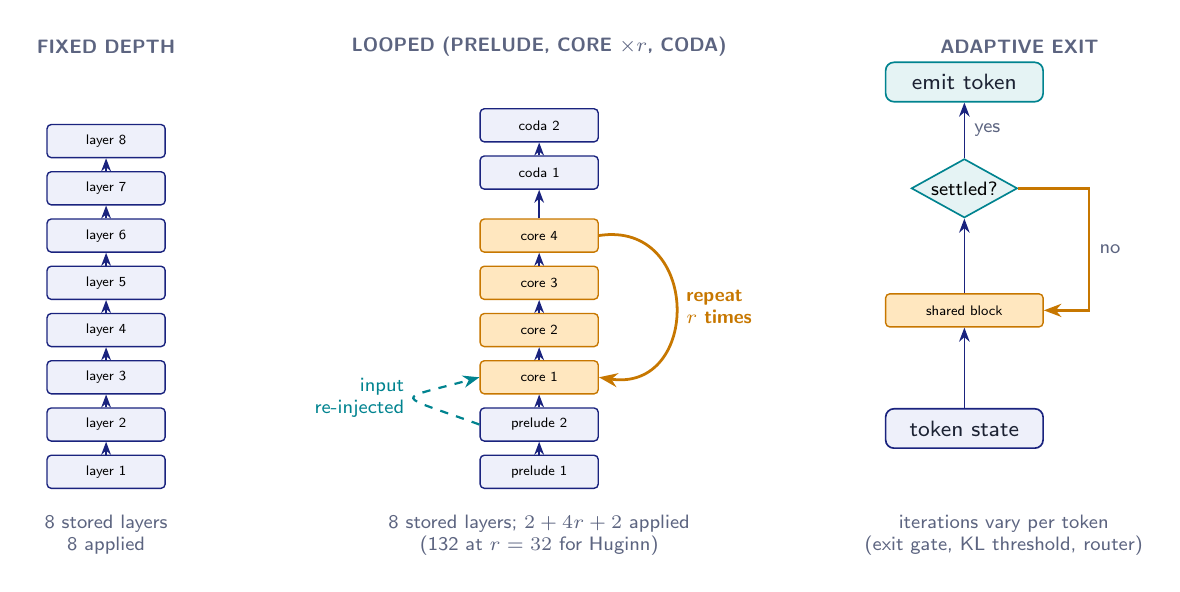
\begin{tikzpicture}[font=\sffamily\footnotesize]
  % Column headers
  \node[colhead] at (1.5,6.35) {FIXED DEPTH};
  \node[colhead] at (7.0,6.35) {LOOPED (PRELUDE, CORE $\times r$, CODA)};
  \node[colhead] at (13.1,6.35) {ADAPTIVE EXIT};
  % Fixed stack
  \foreach \i in {1,...,8} {
    \node[layer, draw=deepindigo, fill=paleindigo] (f\i) at (1.5,0.35+\i*0.6) {layer \i};
  }
  \foreach \i [evaluate=\i as \j using int(\i+1)] in {1,...,7} { \draw[arr, line width=0.5pt] (f\i) -- (f\j); }
  \node[lbl, align=center] at (1.5,0.15) {8 stored layers\\8 applied};
  % Looped
  \node[layer, draw=deepindigo, fill=paleindigo] (p1) at (7.0,0.95) {prelude 1};
  \node[layer, draw=deepindigo, fill=paleindigo] (p2) at (7.0,1.55) {prelude 2};
  \foreach \i in {1,...,4} {
    \node[layer, draw=darkamber, fill=honeyamber!25] (c\i) at (7.0,1.55+\i*0.6) {core \i};
  }
  \node[layer, draw=deepindigo, fill=paleindigo] (d1) at (7.0,4.75) {coda 1};
  \node[layer, draw=deepindigo, fill=paleindigo] (d2) at (7.0,5.35) {coda 2};
  \draw[arr, line width=0.5pt] (p1) -- (p2);
  \draw[arr, line width=0.5pt] (p2) -- (c1);
  \foreach \i [evaluate=\i as \j using int(\i+1)] in {1,...,3} { \draw[arr, line width=0.5pt] (c\i) -- (c\j); }
  \draw[arr, line width=0.5pt] (c4) -- (d1);
  \draw[arr, line width=0.5pt] (d1) -- (d2);
  \draw[aarr, line width=1.0pt] (c4.east) .. controls +(1.3,0.2) and +(1.3,-0.2) .. node[right, font=\sffamily\scriptsize\bfseries, text=darkamber, align=left] {repeat\\$r$ times} (c1.east);
  \draw[darr, draw=sensorteal] (p2.west) .. controls +(-1.1,0.4) and +(-1.1,-0.3) .. node[left, font=\sffamily\scriptsize, text=sensorteal, align=right] {input\\re-injected} (c1.west);
  \node[lbl, align=center] at (7.0,0.15) {8 stored layers; $2+4r+2$ applied\\(132 at $r=32$ for Huginn)};
  % Adaptive
  \node[layer, draw=darkamber, fill=honeyamber!25, minimum width=2.0cm] (a1) at (12.4,3.0) {shared block};
  \node[diamond, aspect=1.8, draw=sensorteal, fill=sensorteal!10, line width=0.6pt, inner sep=1pt, font=\sffamily\scriptsize, align=center] (g) at (12.4,4.55) {settled?};
  \node[observe, minimum width=2.0cm, minimum height=0.5cm] (o) at (12.4,5.9) {emit token};
  \node[flowstep, minimum width=2.0cm, minimum height=0.5cm] (in) at (12.4,1.5) {token state};
  \draw[arr, line width=0.6pt] (in) -- (a1);
  \draw[arr, line width=0.6pt] (a1) -- (g);
  \draw[arr, line width=0.6pt] (g) -- node[right, lbl] {yes} (o);
  \draw[aarr, line width=0.9pt] (g.east) -- ++(0.9,0) |- node[pos=0.25, right, lbl] {no} (a1.east);
  \node[lbl, align=center] at (12.9,0.15) {iterations vary per token\\(exit gate, KL threshold, router)};
\end{tikzpicture}
\caption[Three per-token computation patterns]{Three per-token computation patterns. A looped model applies more layers than it stores, so its weights look shallow; an adaptive one also varies its iterations per token, which is what timing probes look for.}
\label{fig:taxonomy}
\end{figure}

\subsection{Confounders That Are Not Recurrence}
\label{sec:confounders}

{\footnotesize
\zebra
\begin{longtable}{L{3.0cm} L{3.6cm} L{9.35cm}}
\rowcolor{deepindigo}
\hd{Technique} & \hd{What it changes} & \hd{Why it confuses detection} \\
\endfirsthead
\rowcolor{deepindigo}
\hd{Technique} & \hd{What it changes} & \hd{Why it confuses detection (continued)} \\
\endhead
\tablefinish
\endlastfoot
Mixture-of-experts & Active parameters per token & Per-token compute can vary with routing; compute is \emph{below} stored parameters, the opposite direction to looping \\
Mixture-of-Depths~[17] & Which tokens a layer processes & Per-token compute varies with content, like adaptive depth, without iteration \\
Early exit~[15,16] & Layers used per token & Latency rises with difficulty, like adaptive looping \\
Speculative decoding~[18] & Tokens accepted per target-model step & Inter-token latency depends on whether the draft and target models agree on the continuation~[32] \\
Multi-token prediction~[57] & Tokens proposed per forward pass & Extra heads used for self-speculation make inter-token latency content-dependent in the same way \\
Batching, queueing, rate limiting & Time waiting for and sharing the GPU; server-side pacing & Latency depends on other traffic and on the provider's throttling, often more than on your request \\
KV and prefix caching & Prefill work for repeated prefixes & Repeated prompt prefixes run faster~[33] \\
Quantization, hardware changes & Cost per layer; which deployment serves you & A provider can change precision or hardware mid-study, shifting latency for reasons unrelated to depth \\
Gateway buffering & When streamed tokens reach the client & Tokens released in bursts hide inter-token timing and add jitter to time to first token \\
Hidden reasoning tokens & Tokens generated but not shown & The most important confounder for ``invisible thinking'': the extra compute is ordinary decoding, billed but not displayed, and not every provider reports it in usage fields \\
\end{longtable}
}

\textbf{How the designs compare.}

{\footnotesize
\zebra
\begin{tabularx}{\textwidth}{L{3.6cm} L{1.5cm} L{2.0cm} L{2.6cm} Y}
\rowcolor{deepindigo}
\hd{Design} & \hd{Weights reused} & \hd{Iterations} & \hd{Unwritten serial steps} & \hd{Detectable from} \\
Fixed-depth transformer & No & 1 & Bounded by $L$ & (baseline) \\
Looped, fixed count & Yes & Fixed & Up to $r$ times the block depth & Config; compute versus capacity \\
Looped, adaptive & Yes & Per token & Varies by token & Config; timing slope; behavior \\
Latent-thought tokens & No & 1 per position & Across hidden positions & Token counts; per-position timing \\
Early exit & No & 1 (shortened) & Fewer than $L$ & Timing (looks adaptive) \\
Hidden reasoning tokens & No & 1 per token & Across hidden tokens & Usage fields; billing \\
\tablefinish
\end{tabularx}\par}

% ============================================================================
% SECTION 3: WHY IT MATTERS
% ============================================================================
\section{Why Architecture Matters for Safety}
\label{sec:why}

\inbrief{The case rests on one mechanism: looping lets a model do more sequential work per token without writing it down. That erodes chain-of-thought monitoring, moves test-time compute out of sight, allows effort to vary invisibly by input, breaks compute accounting based on parameter counts, and strains interpretability tools built for fixed stacks. Some of this is documented and some is reasoned inference; each claim's strength is marked.}

\subsection{Chain-of-Thought Monitoring}

A 2025 position paper by researchers across several labs argued that chain-of-thought monitoring is ``a new and fragile opportunity'': for hard tasks, models must reason in tokens, and those tokens can be read by a monitor~[27]. The paper names latent reasoning in continuous spaces as one way the window could close. \mO\ OpenAI researchers showed that a monitor reading the chain of thought catches reward hacking more effectively than one watching actions alone, and that optimizing against the monitor teaches models to hide intent~[28]. \mO\ Emmons et al. found that when chain of thought is necessary for a task, models struggle to evade monitors without substantial help~[29]. \mO

The link to architecture follows from theory (Section~\ref{sec:theory}): a fixed-depth transformer \emph{needs} tokens to run long serial computations, which is what makes those computations visible. A looped model can run some of them internally~[19] (Figure~\ref{fig:hidden}). \mE\ Recurrence does not make monitoring impossible: the amount of hidden computation is bounded by loop count times block depth, and intermediate loop states may be decodable (Section~\ref{sec:converge}). It does move the boundary of what must be verbalized.

\begin{figure}[htbp]
\centering
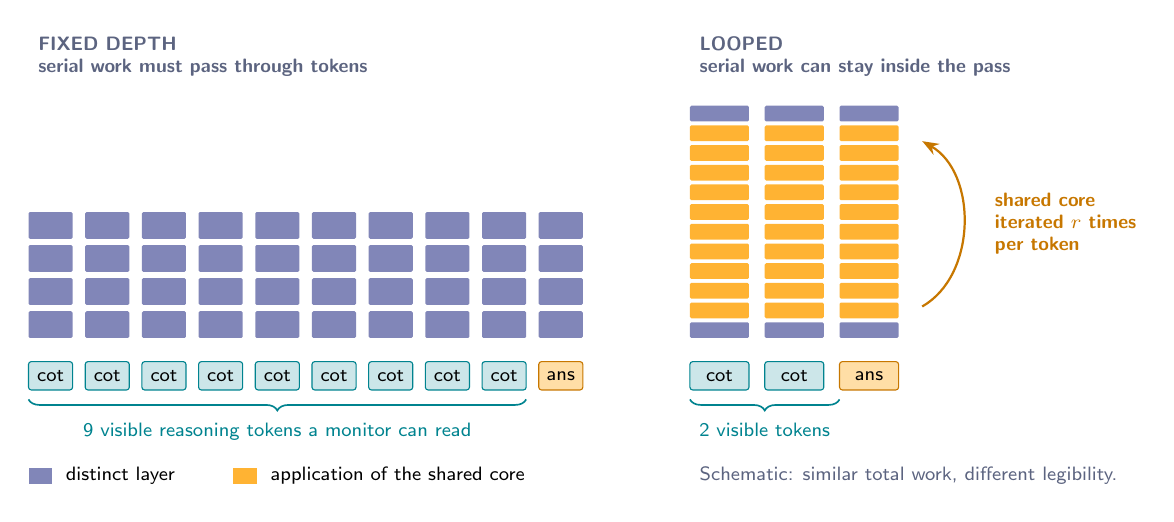
\begin{tikzpicture}[font=\sffamily\scriptsize, x=1cm, y=1cm]
  % Fixed-depth model with visible CoT
  \node[colhead, anchor=south west, align=left] at (0,4.3) {FIXED DEPTH\\serial work must pass through tokens};
  \foreach \t in {0,...,9} {
    \foreach \l in {0,...,3} { \fill[deepindigo!55, rounded corners=0.5pt] (\t*0.72,1.1+\l*0.42) rectangle ++(0.56,0.34); }
    \pgfmathsetmacro{\isans}{\t==9 ? 1 : 0}
    \ifnum\t<9
      \node[rectangle, rounded corners=1pt, fill=sensorteal!20, draw=sensorteal, line width=0.4pt, minimum width=0.56cm, minimum height=0.36cm, inner sep=0pt] at (\t*0.72+0.28,0.62) {cot};
    \else
      \node[rectangle, rounded corners=1pt, fill=honeyamber!35, draw=darkamber, line width=0.4pt, minimum width=0.56cm, minimum height=0.36cm, inner sep=0pt] at (\t*0.72+0.28,0.62) {ans};
    \fi
  }
  \draw[decorate, decoration={brace, amplitude=4pt, mirror}, sensorteal, line width=0.6pt] (0,0.32) -- (6.32,0.32) node[midway, below=5pt, text=sensorteal] {9 visible reasoning tokens a monitor can read};
  % Looped model
  \node[colhead, anchor=south west, align=left] at (8.4,4.3) {LOOPED\\serial work can stay inside the pass};
  \foreach \t in {0,1,2} {
    \foreach \l in {0,...,11} {
      \ifnum\l<1
        \fill[deepindigo!55, rounded corners=0.5pt] (8.4+\t*0.95,1.1+\l*0.25) rectangle ++(0.75,0.2);
      \else\ifnum\l>10
        \fill[deepindigo!55, rounded corners=0.5pt] (8.4+\t*0.95,1.1+\l*0.25) rectangle ++(0.75,0.2);
      \else
        \fill[honeyamber!80, rounded corners=0.5pt] (8.4+\t*0.95,1.1+\l*0.25) rectangle ++(0.75,0.2);
      \fi\fi
    }
  }
  \node[rectangle, rounded corners=1pt, fill=sensorteal!20, draw=sensorteal, line width=0.4pt, minimum width=0.75cm, minimum height=0.36cm, inner sep=0pt] at (8.775,0.62) {cot};
  \node[rectangle, rounded corners=1pt, fill=sensorteal!20, draw=sensorteal, line width=0.4pt, minimum width=0.75cm, minimum height=0.36cm, inner sep=0pt] at (9.725,0.62) {cot};
  \node[rectangle, rounded corners=1pt, fill=honeyamber!35, draw=darkamber, line width=0.4pt, minimum width=0.75cm, minimum height=0.36cm, inner sep=0pt] at (10.675,0.62) {ans};
  \draw[aarr, line width=0.8pt] (11.35,1.5) .. controls +(0.7,0.4) and +(0.7,-0.4) .. (11.35,3.6);
  \node[text=darkamber, anchor=west, align=left, font=\sffamily\scriptsize\bfseries] at (12.15,2.55) {shared core\\iterated $r$ times\\per token};
  \draw[decorate, decoration={brace, amplitude=4pt, mirror}, sensorteal, line width=0.6pt] (8.4,0.32) -- (10.3,0.32) node[midway, below=5pt, text=sensorteal] {2 visible tokens};
  % legend
  \fill[deepindigo!55] (0,-0.75) rectangle ++(0.3,0.2); \node[anchor=west] at (0.35,-0.65) {distinct layer};
  \fill[honeyamber!80] (2.6,-0.75) rectangle ++(0.3,0.2); \node[anchor=west] at (2.95,-0.65) {application of the shared core};
  \node[anchor=west, text=softslate] at (8.4,-0.65) {Schematic: similar total work, different legibility.};
\end{tikzpicture}
\caption[Where serial computation lives]{Where serial computation lives. A fixed-depth model must externalize long chains as tokens; a looped model can keep more of the chain inside each token's forward pass.}
\label{fig:hidden}
\end{figure}

\subsection{Test-Time Compute Inside the Forward Pass}

Reasoning models scale capability by generating more tokens. Recurrent-depth models offer a second axis: more iterations per token~[4,5]. Huginn's accuracy on harder tasks keeps improving with more iterations, while easier tasks saturate sooner (around 8 to 12 iterations in the authors' zero-shot setting)~[4]. \mO\ \mE\ Compute spent this way is invisible to anyone counting tokens, and on an API it may not show up in usage or billing.

\subsection{Invisible, Selective Effort}

With adaptive depth, the model decides how much to compute per token. Huginn's own analysis shows that it already varies effort by content: exits come later on moral-scenario questions than on high-school mathematics, by about 3.5 steps on average~[4]. \mO

\mS\ A model with situational awareness could in principle spend extra hidden computation on inputs it recognizes as evaluations, or spend less while appearing to try (sandbagging), without any trace in its visible reasoning. There is no public evidence of a looped model doing this. The concern is that the mechanism for content-dependent hidden effort exists, and that evaluation awareness in frontier models is rising (Section~\ref{sec:astra}), so the two together deserve measurement rather than assumption.

\subsection{Compute Accounting and Thresholds}

Governance frameworks use compute as a proxy for capability. The EU AI Act presumes that a general-purpose model has high-impact capabilities when cumulative training compute exceeds $10^{25}$ floating-point operations~[56]. \mO\ \mE\ Training compute that is measured directly is unaffected by looping. Compute that is \emph{estimated} from parameter count and tokens (the common $6ND$ rule of thumb) undercounts a looped model by roughly its loop factor, because each stored parameter is used $r$ times per token. Inference compute becomes input-dependent under adaptive depth, so thresholds and evaluations framed in per-token cost are moving targets. Disclosure of loop counts (Section~\ref{sec:recs}) closes this gap; external estimation can only bound it.

\subsection{Interpretability Transfer}

Tools such as the logit lens~[37], the tuned lens~[38], probing, and layer-wise representation similarity~[39] assume a fixed layer index. In a looped model, ``layer 3'' is visited $r$ times with different meanings. Lu et al. applied logit-lens and coda-lens probing to Huginn and found only limited evidence of interpretable latent chain of thought, with more recurrence giving marginal gains on their arithmetic tasks~[40]. \mO\ \mE\ Tools need to be re-indexed by iteration, and their validity re-established, before their outputs on looped models are trusted.

\subsection{Case Study: the 2026 Astra Reports}
\label{sec:astra}

This episode shows why external detection matters and why it must stay calibrated. Every architecture claim in it comes from reporting or from developer statements that neither confirm nor exclude looping; the measurements come from the system card.

{\footnotesize
\zebra
\begin{longtable}{L{1.45cm} L{10.6cm} L{3.9cm}}
\rowcolor{deepindigo}
\hd{Date (2026)} & \hd{Event} & \hd{Status} \\
\endfirsthead
\rowcolor{deepindigo}
\hd{Date (2026)} & \hd{Event (continued)} & \hd{Status} \\
\endhead
\tablefinish
\endlastfoot
1 Sep & \emph{The Information} (A.~Efrati) reports, citing a person with knowledge, that OpenAI's Astra model uses ``recurrent depth'', also called a looped transformer, and that OpenAI limits its use to keep the chain of thought legible~[55] & Reported; paywalled, not read directly here; relayed by [51,53,58] \\
2 Sep & OpenAI chief scientist Jakub Pachocki posts that ``The depth of the computation graph for our present frontier models, including Astra, is within a factor of two of GPT-4'' and that he wants ``to prevent a race into unmonitorability kicked off by confused reporting''~[52] & Developer statement, quoted as reproduced in [53,54]; neither confirms nor rules out limited looping \\
3 Sep & Fortune, paraphrasing OpenAI researchers, reports that OpenAI ``had limited the extent to which the looped Transformer architecture is used so that the model's reasoning remains legible''; Daniel Kokotajlo urges an industrywide standard on CoT monitorability~[51] & Reported characterization; implies partial use \\
3 Sep & The GPT-6 Astra system card (revised 9, 22, and 29 September) states that ``GPT-6 Astra's monitorability has decreased relative to GPT-5.6 Sol'' and that OpenAI is ``quite confident that changes in CoT controllability are not differentially due to any architectural changes''~[50] & Primary source; architecture not described \\
6 Sep & Pachocki's essay ``An Alien Mind'' says no lab has solved alignment and monitoring well enough to keep scaling at maximum speed for much longer, and that OpenAI would ``unilaterally withhold further scaling as needed''~[60] & Developer statement, quoted from press reproductions \\
28--29 Sep & OpenAI delays GPT-6.1 Astra after safety testing; Saachi Jain is quoted as saying it ``didn't quite meet the bar'' on staying within scope and authorization~[61] & Reported (WSJ, via AFP) \\
1--9 Oct & The WSJ reports that OpenAI has dismissed three safety researchers for violating its policies on handling sensitive information~[62]; on 9 October OpenAI says the firings ``were not about safety concerns or speaking out'', and the researchers dispute its account~[63] & Reported; contested \\
13--15 Oct & \emph{The Information} reports that OpenAI is working to fix safety issues before shipping its next flagship model; secondary coverage links that model to a looped transformer~[64] & Secondary; architecture unconfirmed \\
\end{longtable}
}

\textbf{What the system card measures.} The card's monitorability and alignment sections give the figures below in their text (see also Figure~\ref{fig:astracard})~[50]. Each row is a different measurement, and values are not comparable across rows.

{\footnotesize
\zebra
\begin{longtable}{L{8.6cm} L{4.4cm} L{2.95cm}}
\rowcolor{deepindigo}
\hd{Measure (card section)} & \hd{Comparison model} & \hd{GPT-6 Astra} \\
\endfirsthead
\rowcolor{deepindigo}
\hd{Measure (card section)} & \hd{Comparison model} & \hd{GPT-6 Astra} \\
\endhead
\tablefinish
\endlastfoot
CoT controllability, OpenAI CoT-Control suite, CoTs of 750--1,250 tokens (9.2.1) & GPT-5.6 Sol 16.1\%; GPT-5.5 Thinking 1.7\% & 60.9\% \\
CoT controllability, UK AISI's own run (9.3) & GPT-5.6 Sol 48\% & 93\% \\
No-CoT time horizon, UK AISI, with a contamination caveat (9.3) & GPT-5.6 Sol 3.6 min & 30.9 min \\
Verbalized evaluation awareness, deployment simulation (8.6) & GPT-5.6 Sol 2.8\% & 9.6\% \\
Verbalized evaluation awareness, Apollo Research, xhigh effort (8.8.1) & GPT-5.5 27.7\% & 41.1\% (50.6\% at max effort) \\
Recall of a CoT-only monitor when the model is told to sandbag and evade (9.2.2.3.1) & GPT-5.6 Sol nearly 100\% & below 11\% \\
\end{longtable}
}

\begin{figure}[htbp]
\centering
\pgfplotsset{
  cardbar/.style={
    ybar=3.5pt, width=5.75cm, height=5.4cm, ymin=0, ymax=105, bar width=7pt,
    axis lines=left, ymajorgrids, grid style={medgray!40},
    tick label style={font=\sffamily\scriptsize}, label style={font=\sffamily\scriptsize},
    title style={font=\sffamily\scriptsize\bfseries, text=deepindigo, align=center},
    x tick label style={font=\sffamily\scriptsize, align=center, text width=2.1cm},
    yticklabel style={/pgf/number format/assume math mode=true, font=\sffamily\scriptsize},
    nodes near coords, nodes near coords style={font=\sffamily\tiny, text=textdark, /pgf/number format/assume math mode=true, /pgf/number format/fixed, /pgf/number format/precision=1},
    legend style={font=\sffamily\tiny, draw=none, fill=none, at={(0.5,-0.24)}, anchor=north, cells={anchor=west}},
    enlarge x limits=0.42, anchor=south west,
  }
}
\begin{tikzpicture}[baseline=0pt]
\begin{axis}[cardbar, title={CoT controllability (\%)\\Astra card 9.2.1 and 9.3}, symbolic x coords={OpenAI suite, UK AISI run}, xtick={OpenAI suite, UK AISI run}]
\addplot[fill=proxygray!70, draw=proxygray] coordinates {(OpenAI suite,1.7)};
\addplot[fill=deepindigo, draw=deepindigo] coordinates {(OpenAI suite,16.1) (UK AISI run,48)};
\addplot[fill=alertcrimson, draw=alertcrimson] coordinates {(OpenAI suite,60.9) (UK AISI run,93)};
\legend{GPT-5.5 Thinking, GPT-5.6 Sol, GPT-6 Astra}
\end{axis}
\end{tikzpicture}\hfill
\begin{tikzpicture}[baseline=0pt]
\begin{axis}[cardbar, ymax=70, title={Verbalized evaluation awareness (\%)\\Astra card 8.6 and 8.8.1}, symbolic x coords={Deployment simulation, Apollo xhigh}, xtick={Deployment simulation, Apollo xhigh}]
\addplot[fill=deepindigo, draw=deepindigo] coordinates {(Deployment simulation,2.8) (Apollo xhigh,27.7)};
\addplot[fill=alertcrimson, draw=alertcrimson] coordinates {(Deployment simulation,9.6) (Apollo xhigh,41.1)};
\legend{predecessor (Sol; GPT-5.5 for Apollo), GPT-6 Astra}
\end{axis}
\end{tikzpicture}\hfill
\begin{tikzpicture}[baseline=0pt]
\begin{axis}[cardbar, ymax=70, title={Unverbalized evaluation awareness (\%)\\Opus 5.5 card 6.6.1, white-box}, symbolic x coords={Automated audits, Real use}, xtick={Automated audits, Real use}]
\addplot[fill=sensorteal, draw=sensorteal] coordinates {(Automated audits,36) (Real use,0.4)};
\legend{Claude Opus 5.5}
\end{axis}
\end{tikzpicture}
\caption[Monitorability measurements from two system cards]{Astra's card reports large rises in CoT controllability and verbalized evaluation awareness over its predecessors; these register the result, not the mechanism (Figure~\ref{fig:attribution}). Values are those stated in the text of the two system cards~[50,65]. Each panel uses its own instrument and units: controllability and verbalized awareness are read from the model's visible reasoning, while the right panel uses white-box readouts of the model's internals. Do not compare bar heights across panels or across labs. Apollo's max-effort figure for Astra is 50.6\%.}
\label{fig:astracard}
\end{figure}

The card also says that Astra is ``substantially better than GPT-5.6 Sol at evading CoT-only monitors, particularly with step-by-step guidance and at lower reasoning effort'', that against a high-recall full-trajectory monitor the ``successful evasion rate is close to zero'', and that ``if the model were to try to sandbag covertly, we would likely be unable to catch it reliably''. UK AISI ``was not able to complete agentic evaluations of Astra's monitorability'', and Apollo Research cautions that, given the model's evaluation awareness, ``low rates of misbehavior here do not provide substantial evidence about the model's alignment or misalignment''. OpenAI states that it ``will not accept further degradation of monitoring beyond a limit, without new ways to demonstrate alignment generalization''~[50]. \mO

Other developers measure related properties with different methods. Anthropic's Claude Opus 5.5 system card (22 September) replicates the controllability evaluation with one point per reasoning-effort level or thinking budget and finds that Opus 5.5 ``controls its CoT about as well as Claude Opus 4.7''; it measures \emph{unverbalized} evaluation awareness with white-box readouts, reporting that 36\% of automated behavioral audit transcripts but only 0.4\% of about 500 internal Claude Code transcripts scored 6 or higher~[65]. \mO\ These are different instruments from OpenAI's, so the two labs' numbers must not be placed on one scale.

\textbf{What follows from this.} \mE\ The developer documents the symptoms: more reasoning fits in one forward pass, the model controls its visible reasoning better, and trace-based monitors catch less. It attributes the change mainly to capability, not architecture. Behavioral monitorability metrics cannot settle that attribution. Controllability, evaluation awareness, and no-CoT time horizon would move the same way whether the extra single-pass capability came from training data and recipes, from more layers, or from loops: they measure the result, not the mechanism (Figure~\ref{fig:attribution}). Commentators split accordingly: Raschka credits mainly ``improved training recipes and training data'', with looping that ``might help a bit''~[53]; Arike guesses ``three to four loops'' and argues that the number of loops ``can then be viewed as a dial that can be turned up with trivial effort''~[54]. Both are opinions, not measurements.

The distinction matters for what comes next. A capability-driven decline would affect every frontier model on roughly the same schedule; an architecture-driven one is a design setting that can be raised across releases, though not freely for every design (Section~\ref{sec:counter}). Only evidence about \emph{how} the model computes separates the two: disclosure of loop counts (Section~\ref{sec:recdev}) or measurements of the kind in Section~\ref{sec:methods}, which ask whether a deployed model's in-pass serial capability, latency, and compute behave like a fixed or a looped model, without needing the weights.

\begin{figure}[htbp]
\centering
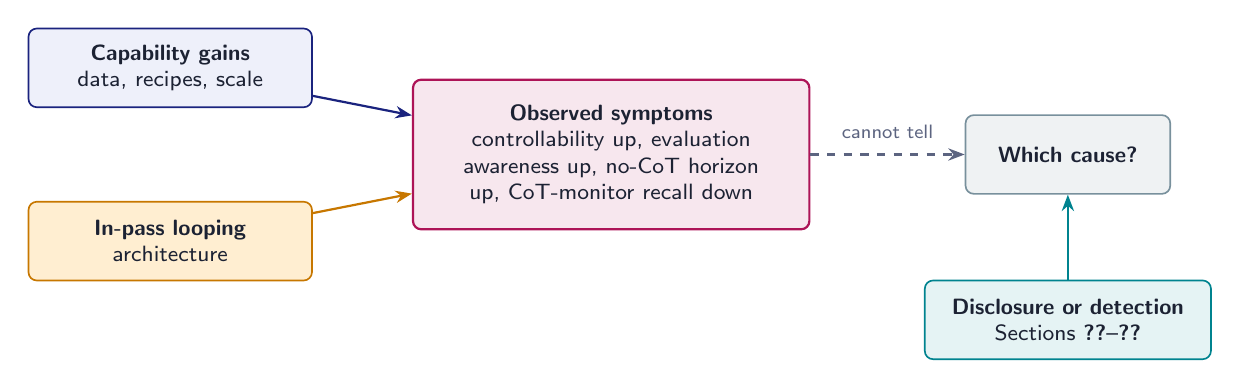
\begin{tikzpicture}[font=\sffamily\footnotesize]
  \node[flowstep, minimum width=3.6cm, minimum height=1.0cm] (cap) at (0,1.1) {\textbf{Capability gains}\\data, recipes, scale};
  \node[loopbox, minimum width=3.6cm, minimum height=1.0cm] (loop) at (0,-1.1) {\textbf{In-pass looping}\\architecture};
  \node[hot, minimum width=5.0cm, text width=4.8cm, minimum height=1.9cm] (sym) at (5.6,0) {\textbf{Observed symptoms}\\controllability up, evaluation awareness up, no-CoT horizon up, CoT-monitor recall down};
  \node[quiet, minimum width=2.6cm, minimum height=1.0cm] (q) at (11.4,0) {\textbf{Which cause?}};
  \node[observe, minimum width=3.6cm, text width=3.4cm, minimum height=1.0cm] (det) at (11.4,-2.1) {\textbf{Disclosure or detection}\\Sections~\ref{sec:methods}--\ref{sec:validation}};
  \draw[arr] (cap) -- (sym);
  \draw[aarr] (loop) -- (sym);
  \draw[darr, draw=softslate] (sym) -- node[above=2pt, lbl] {cannot tell} (q);
  \draw[arr, draw=sensorteal] (det) -- (q);
\end{tikzpicture}
\caption[Why behavioral metrics cannot attribute the decline]{Why behavioral metrics cannot attribute a monitorability decline. Both causes produce the same symptoms; separating them needs disclosure or architecture-level evidence.}
\label{fig:attribution}
\end{figure}

\subsection{The Counter-Case}
\label{sec:counter}

Looping has real benefits, and the risk case is partly speculative:
\begin{itemize}
  \item \textbf{Efficiency.} Fewer parameters for the same reasoning means cheaper deployment and smaller models that fit on local hardware~[5,14].
  \item \textbf{Faithfulness claims.} Ouro's authors report that LoopLM reasoning traces align more closely with final outputs than explicit chain of thought, and that harmfulness on the HEx-PHI benchmark falls as recurrent steps increase~[5]. \mO\ These are the authors' measurements, not yet independently replicated.
  \item \textbf{Bounded hidden computation.} Serial depth per token is still bounded by loop count times block depth; there is no unbounded hidden state carried across tokens as in a classic RNN. \mE
  \item \textbf{Possible readability.} Intermediate loop states can be decoded through the coda or a lens, and Ouro's design produces a valid next-token distribution at every step~[5,40]. \mO\ Whether those readouts are faithful enough to monitor is open.
  \item \textbf{Saturation.} Ouro's accuracy \emph{falls} when run beyond its trained four steps (the 2.6B Thinking model drops from 76.44 at four steps to 39.26 at eight on OlympiadBench)~[5], so ``turn the dial up'' is not free for every design. \mO
\end{itemize}

\begin{notebox}[Balanced reading]
Looping is a capability and efficiency technique with a specific monitoring cost. The cost is real in mechanism and documented in its symptoms (Section~\ref{sec:astra}), but which deployed systems carry it, and how much, is not publicly known. That is the gap this guide addresses.
\end{notebox}

% ============================================================================
% SECTION 4: THEORY
% ============================================================================
\section{What Theory and Evidence Say About Serial Depth}
\label{sec:theory}

\inbrief{Theory says fixed-depth transformers cannot solve some sequential problems in one pass, and that looping or chain of thought lifts the limit. Those same problems make the behavioral probes of Section~\ref{sec:behavior}.}

\begin{itemize}
  \item \textbf{Fixed depth is limited.} Hahn proved that self-attention cannot model periodic finite-state languages (parity is the classic case) or hierarchical structure unless layers or heads grow with input length~[26]. Merrill, Petty, and Sabharwal showed that transformers and state-space models alike cannot solve state tracking such as permutation composition for long sequences~[25]. \mO
  \item \textbf{Chain of thought helps in proportion to its length.} Intermediate generation extends a transformer's power by an amount that depends on the number of steps~[23]. \mO
  \item \textbf{Depth growth helps too.} Transformers whose depth grows logarithmically with input length can recognize regular languages and solve graph connectivity, which fixed-depth ones cannot under standard conjectures~[24]. \mO
  \item \textbf{Loops can stand in for tokens.} A $k$-layer transformer looped $L$ times nearly matches a $kL$-layer model on reasoning tasks (addition, $p$-hop induction, math); looped models can simulate $T$ steps of chain of thought with $T$ loops; and looping helps reasoning far more than memorization~[19]. Looped transformers can emulate programmable computers~[20], learn learning algorithms with under 10\% of the parameters~[21], and generalize to longer inputs when the step count adapts~[22]. \mO
  \item \textbf{Language models already do some latent multi-hop reasoning}, with strength that varies by relation~[49]. \mO
\end{itemize}

\textbf{Implication for detection.} \mE\ Ask problems whose serial depth you control, in a format that forbids writing steps out. A fixed-depth model's accuracy should fall as depth passes what its layers can do in one pass; a looped model's should hold up longer; an adaptive one should spend more time on deeper items. Accuracy curves alone confound depth with scale (a larger fixed model also holds up longer), as Figure~\ref{fig:depthcurves} shows, which is why Section~\ref{sec:scoring} never lets behavior decide alone.

\begin{figure}[htbp]
\centering
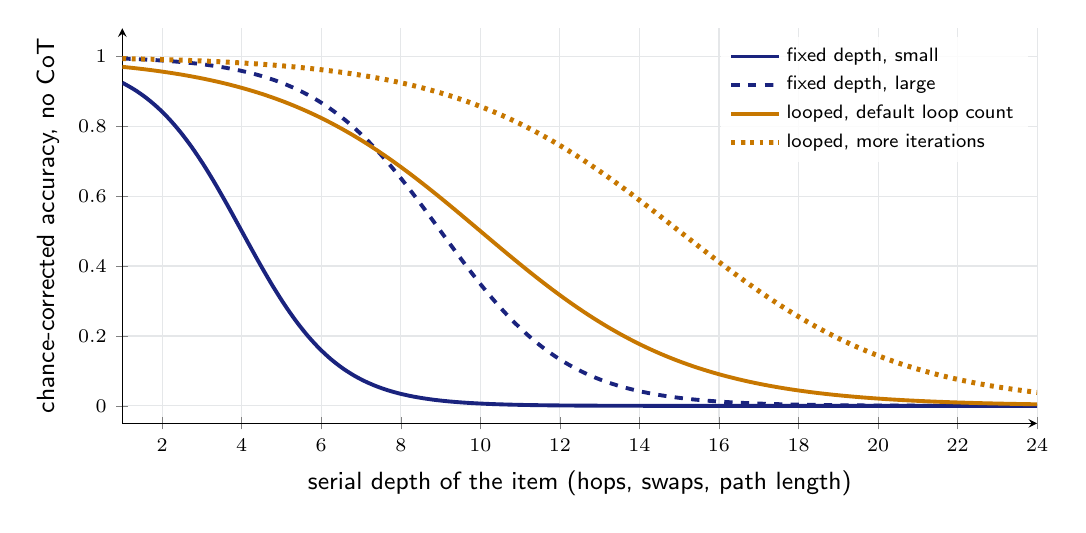
\begin{tikzpicture}
\begin{axis}[
  width=13.2cm, height=6.6cm,
  xmin=1, xmax=24, ymin=-0.05, ymax=1.08,
  xlabel={serial depth of the item (hops, swaps, path length)},
  ylabel={chance-corrected accuracy, no CoT},
  label style={font=\sffamily\small}, tick label style={font=\sffamily\scriptsize},
  axis lines=left, grid=major, grid style={medgray!40},
  legend style={font=\sffamily\scriptsize, draw=none, fill=white, fill opacity=0.85, text opacity=1, at={(0.99,0.98)}, anchor=north east, cells={anchor=west}},
  every axis plot/.append style={line width=1.4pt, samples=80, smooth}
]
\addplot[deepindigo, domain=1:24] {1/(1+exp(-(4-x)/1.2))};
\addlegendentry{fixed depth, small}
\addplot[deepindigo, dashed, domain=1:24] {1/(1+exp(-(9-x)/1.6))};
\addlegendentry{fixed depth, large}
\addplot[darkamber, domain=1:24] {1/(1+exp(-(10-x)/2.6))};
\addlegendentry{looped, default loop count}
\addplot[darkamber, dotted, line width=1.8pt, domain=1:24] {1/(1+exp(-(15-x)/2.8))};
\addlegendentry{looped, more iterations}
\end{axis}
\end{tikzpicture}
\caption[Schematic accuracy against controlled serial depth]{Schematic accuracy against controlled serial depth (illustrative curves, not data). A large fixed-depth model and a looped model can produce similar curves, so behavior alone confounds depth with scale; the shape of accuracy against an iteration or budget setting is more diagnostic.}
\label{fig:depthcurves}
\end{figure}

% ============================================================================
% PART II
% ============================================================================
\partbanner{II}{Detection}{Methods by access level, their confounders, and how to combine them into a calibrated verdict}{%
  % three tiers converging on a verdict
  \foreach \y/\c/\w in {5.8/sensorteal/3.4, 3.9/indigo/2.6, 2.0/honeyamber/1.8} {
    \fill[\c, opacity=0.65, rounded corners=2pt] (0.3,\y) rectangle ++(\w,0.7);
    \draw[white, opacity=0.5, line width=0.9pt, -{Stealth[scale=1.0]}] (0.45+\w,\y+0.35) -- (5.3,3.9);
  }
  \fill[white, opacity=0.9, rounded corners=3pt] (5.4,3.35) rectangle ++(2.4,1.1);
  \node[font=\sffamily\scriptsize\bfseries, text=nightink, align=center] at (6.6,3.9) {recurrent\\fixed\\inconclusive};
}

% ============================================================================
% SECTION 5: METHODS
% ============================================================================
\section{Detection Methods by Access Level}
\label{sec:methods}

\inbrief{Each method is described by the signal it yields, its confounders, and its evidence strength. White-box methods observe; gray- and black-box methods infer.}

\subsection{Overview}

Figure~\ref{fig:glance} condenses this table; the table adds the signal each method yields and the methods that only set context.

{\footnotesize
\zebra
\begin{longtable}{L{3.3cm} L{1.2cm} L{3.8cm} L{4.3cm} L{2.5cm}}
\rowcolor{deepindigo}
\hd{Method} & \hd{Access} & \hd{Signal} & \hd{Main confounders} & \hd{Strength} \\
\endfirsthead
\rowcolor{deepindigo}
\hd{Method} & \hd{Access} & \hd{Signal} & \hd{Main confounders} & \hd{Strength} \\
\endhead
\tablefinish
\endlastfoot
Config and code inspection & White & Declared loop count, exit settings & Custom code that loops without declaring it & Decisive when positive \\
Exact or low-rank layer sharing & White & Duplicate or low-rank-related layer weights & Pruned or merged models & Strong \\
Declared versus stored depth & White & Fewer distinct layers than declared & Export quirks & Strong \\
Hidden-state convergence & White & Contraction toward a fixed point across iterations & Normalization effects & Moderate \\
Logit-lens settling & White & Per-token step at which predictions stop changing & Early-exit models settle too & Moderate \\
Width from log-probabilities & Gray & Hidden size & (descriptive, not diagnostic alone) & Context only \\
Compute-to-capacity ratio & Gray & Compute per token above stored capacity & Every input is a rough estimate & Weak \\
TTFT and inter-token slope & Black & Latency rises with serial depth at fixed length & Batching, queueing, early exit, MoD, speculative decoding & Moderate if controlled \\
Serial-depth retention & Black & No-CoT accuracy holds as depth grows & Model scale, training data & Weak alone \\
Compute knob sensitivity & Black & Latency and accuracy rise with a budget setting without extra tokens & Hidden reasoning tokens; routing to another model & Moderate \\
Family fingerprinting~[35,36] & Black & Which known model family an endpoint resembles & Fine-tuning, system prompts & Context (sets the prior) \\
\end{longtable}
}

\subsection{White Box: Open Weights}
\label{sec:whitebox}

\subsubsection{Config and code}
\label{sec:config}

Looped models must tell their modeling code how many iterations to run. In the published configs, Huginn declares \cfg{mean\_recurrence} (32) and \cfg{n\_layers\_in\_recurrent\_block} (4) alongside prelude and coda sizes, for an effective depth of 132; Ouro declares \cfg{total\_ut\_steps} (4) and \cfg{early\_exit\_threshold}; ALBERT declares layer-group sharing with \cfg{num\_hidden\_groups}~[4,5]. Nanbeige4.2-3B declares \cfg{num\_loops} (2)~[59]. \mO\ The toolkit's \cfg{inspect-config} classified all eight published configs it was run on correctly (Section~\ref{sec:results}), and flags Nanbeige's published fields as looped (44 layer applications from 22 stored layers).

Absence is weak evidence. A config can omit recurrence if custom modeling code loops anyway; such code is loaded through the \cfg{auto\_map} field and requires \cfg{trust\_remote\_code}. Read the forward method: a loop over a shared module, or a module list that repeats the same object, is decisive.

\subsubsection{Parameter sharing in the weights}
\label{sec:sharing}

Three patterns, in decreasing order of directness:
\begin{enumerate}
  \item \textbf{Exact duplicates or missing slots.} Two layer slots hold byte-identical tensors, which happens when an export clones a shared block once per use. Hugging Face \cfg{save\_pretrained} instead refuses to write aliased tensors to safetensors and drops the duplicate names, so a module list that repeats one module object usually appears as a stack with \emph{missing} indices. The toolkit reports both; gaps also come from pruning, so they prompt a reading of the code rather than a verdict.
  \item \textbf{Low-rank relation.} The difference between two layers is low rank, as in a shared base matrix plus per-layer LoRA deltas~[7]. Independent trained layers have full-rank differences: on SmolLM2-135M, adjacent layers' weight matrices are 1.32 to 1.41 apart in relative Frobenius distance, close to the $\sqrt{2}$ expected for unrelated matrices of equal norm (Section~\ref{sec:results}).
  \item \textbf{Storage-level reuse.} \mO/\mE\ A block that is looped is stored once. Huginn's checkpoint stores 8 layers; Ouro-1.4B stores 24 and runs them up to four times. Weight files alone therefore look like a shallow model, and only the config, the code, or a compute-versus-capacity mismatch reveals the looping. For the same reason the scorer treats weight-sharing signals as one-sided: their presence is strong evidence of recurrence, their absence only weak evidence against (Section~\ref{sec:llr}).
\end{enumerate}

\subsubsection{Representation similarity}
\label{sec:similarity}

Layer-by-layer similarity matrices (cosine or linear CKA~[39]) show block structure in most models; Gromov et al. and Lad et al. document how redundant many deeper layers are~[47,48]. A repeated block can produce a periodic pattern in such matrices. The toolkit measures this as excess similarity at one lag over its neighbors; on SmolLM2-135M the excess is 0.002, effectively none. \mE\ This is a heuristic: weight reuse does not guarantee repeated representations, so treat it as supporting evidence only.

\subsubsection{Iterate the core and watch it converge}
\label{sec:converge}

The most informative activation test runs the suspected core block repeatedly and records the state after each iteration (Figure~\ref{fig:converge}).
\begin{itemize}
  \item Huginn's authors report that many tokens' states converge to a fixed point, some fall into orbits on harder problems, and some drift steadily in one direction (``sliders''), possibly acting as counters~[4]. \mO
  \item A fixed-depth model has no reason to converge across layers: on SmolLM2-135M the ratio of successive relative state changes over the last half of the stack is 1.12, not contracting (Section~\ref{sec:results}).
  \item Logit-lens decoding~[37] of each iteration gives a per-token \emph{settling step}, the iteration after which the decoded distribution stops changing. Huginn uses exactly this quantity (KL below $5\times10^{-4}$) as its exit rule~[4]. Wide variation in settling steps across tokens, correlated with difficulty, is direct evidence of adaptive depth.
\end{itemize}

\begin{figure}[htbp]
\centering
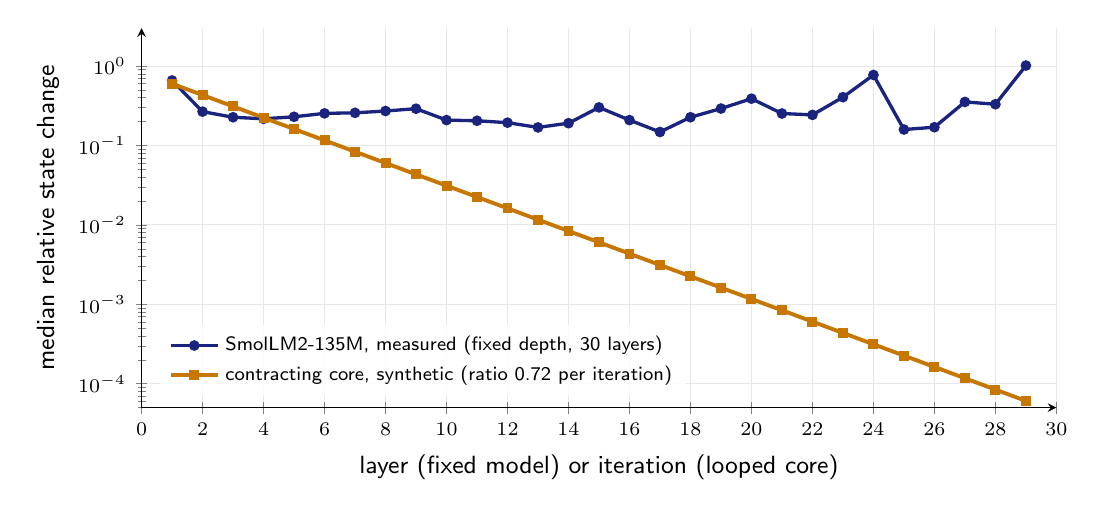
\begin{tikzpicture}
\begin{semilogyaxis}[
  width=13.2cm, height=6.4cm,
  xmin=0, xmax=30, ymin=0.00005, ymax=3,
  xlabel={layer (fixed model) or iteration (looped core)},
  ylabel={median relative state change},
  label style={font=\sffamily\small}, tick label style={font=\sffamily\scriptsize},
  axis lines=left, grid=major, grid style={medgray!40},
  legend style={font=\sffamily\scriptsize, draw=none, fill=white, fill opacity=0.85, text opacity=1, at={(0.02,0.03)}, anchor=south west, cells={anchor=west}},
]
\addplot[deepindigo, line width=1.2pt, mark=*, mark size=1.3pt] coordinates {
(1,0.659) (2,0.267) (3,0.227) (4,0.217) (5,0.230) (6,0.254) (7,0.258) (8,0.272) (9,0.291) (10,0.209)
(11,0.205) (12,0.194) (13,0.169) (14,0.191) (15,0.302) (16,0.209) (17,0.148) (18,0.227) (19,0.292) (20,0.389)
(21,0.253) (22,0.243) (23,0.406) (24,0.774) (25,0.159) (26,0.170) (27,0.354) (28,0.331) (29,1.016)};
\addlegendentry{SmolLM2-135M, measured (fixed depth, 30 layers)}
\addplot[darkamber, line width=1.4pt, domain=1:29, samples=29, mark=square*, mark size=1.1pt] {0.6*0.72^(x-1)};
\addlegendentry{contracting core, synthetic (ratio 0.72 per iteration)}
\end{semilogyaxis}
\end{tikzpicture}
\caption[State change per step: fixed stack versus contracting core]{Convergence is the white-box signature of a looped core. The measured fixed-depth curve comes from the toolkit run on SmolLM2-135M (48 tokens) and shows no decay (tail ratio 1.12). The contracting curve is synthetic, illustrating the geometric decay toward a fixed point that Geiping et al. report for many Huginn tokens.}
\label{fig:converge}
\end{figure}

\begin{warnbox}[Repeating a fixed model's layer is a weak control]
Fixed-depth models tolerate deleting, swapping, and sometimes duplicating middle layers~[47,48]. A layer that survives being repeated is not evidence of recurrent training. The contrast that matters is \emph{convergence} under iteration, not mere robustness.
\end{warnbox}

\subsection{Gray Box: Log-Probabilities}
\label{sec:graybox}

\begin{itemize}
  \item \textbf{Width.} The final layer maps a $d$-dimensional state to the vocabulary, so logit vectors from many prompts span at most $d$ dimensions. Carlini et al. used this to confirm hidden sizes of 1024 and 2048 for OpenAI's Ada and Babbage models~[30]; Finlayson et al. estimated gpt-3.5-turbo's embedding size at about 4096 and showed the same ``model image'' can detect model updates and identify the source model~[31]. \mO\ Width alone says nothing about looping.
  \item \textbf{Compute-to-capacity ratio.} \mS\ Combine an estimate of compute per token (from decode latency on known hardware, or a published figure) with an estimate of stored capacity (from width, a published size, or memorization probes). Looping pushes compute above what the stored parameters would cost once; mixture-of-experts pushes it below. Ouro's authors report that looped and non-looped models store knowledge similarly, so the advantage comes from knowledge manipulation rather than capacity~[5], which is what makes capacity a usable denominator in principle. Every input has wide error bars; the toolkit caps this signal low.
  \item \textbf{Use limits.} Section~\ref{sec:guardrails} restricts this to vectors you are entitled to collect, at the rate limits you are given, and to estimating one shape parameter, never weights.
\end{itemize}

\subsection{Black Box: API Access}
\label{sec:blackbox}

\subsubsection{Timing}
\label{sec:timing}

\textbf{Hypothesis.} \mE\ With adaptive per-token depth, items needing more serial steps should get more iterations, so the time to first token (TTFT) and the inter-token latency (ITL) should rise with serial depth even when prompt and output lengths are identical. With a fixed-depth dense model they should not (Figure~\ref{fig:ttft}).

\textbf{Design controls.}
\begin{itemize}
  \item \textbf{Constant length.} The toolkit's task generators keep prompt length identical across depths within each family (fixed-width fields, identity operations written in the same form as real ones, fixed edge counts) and cap the output at a few tokens.
  \item \textbf{Interleaving.} All conditions are shuffled into one seeded random order, so drift in server load spreads across depths.
  \item \textbf{Log scale and pooling.} Regress log latency on depth (with prompt tokens as a covariate when they vary), trim the slowest 5\% per family, and pool families by inverse variance. The result is a $z$-score.
  \item \textbf{Exclusion of hidden tokens.} Requests whose usage reports reasoning tokens are dropped: hidden decoding is the most likely non-architectural cause of a latency slope. Where a provider does not report them, the toolkit also expresses the TTFT increase across the depth range in units of the median inter-token latency. Extra loop iterations on the first token cost a fraction of one decode step each, so an increase worth tens of tokens points to hidden decoding or routing, not looping. \mE
\end{itemize}

\begin{figure}[htbp]
\centering
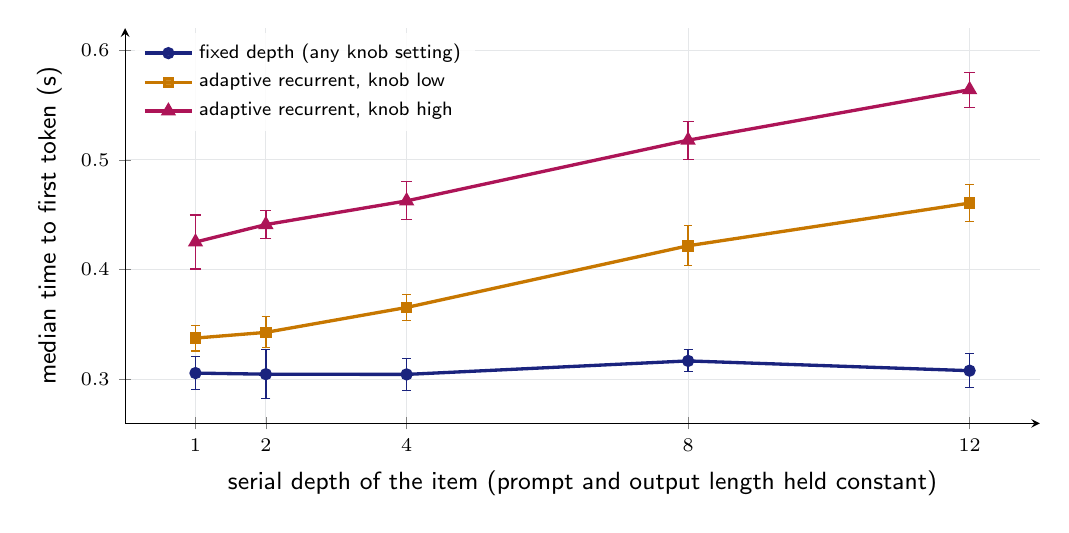
\begin{tikzpicture}
\begin{axis}[
  width=13.2cm, height=6.6cm,
  xmin=0, xmax=13, ymin=0.26, ymax=0.62,
  xtick={1,2,4,8,12},
  xlabel={serial depth of the item (prompt and output length held constant)},
  ylabel={median time to first token (s)},
  label style={font=\sffamily\small}, tick label style={font=\sffamily\scriptsize},
  axis lines=left, grid=major, grid style={medgray!40},
  legend style={font=\sffamily\scriptsize, draw=none, fill=white, fill opacity=0.85, text opacity=1, at={(0.01,0.99)}, anchor=north west, cells={anchor=west}},
  error bars/y dir=both, error bars/y explicit,
]
\addplot[deepindigo, line width=1.2pt, mark=*, mark size=1.6pt, error bars/error bar style={deepindigo, line width=0.6pt}] coordinates {
(1,0.3058) +- (0,0.0149) (2,0.3048) +- (0,0.0221) (4,0.3046) +- (0,0.0149) (8,0.3169) +- (0,0.0100) (12,0.3080) +- (0,0.0154)};
\addlegendentry{fixed depth (any knob setting)}
\addplot[darkamber, line width=1.2pt, mark=square*, mark size=1.5pt, error bars/error bar style={darkamber, line width=0.6pt}] coordinates {
(1,0.3377) +- (0,0.0118) (2,0.3429) +- (0,0.0141) (4,0.3656) +- (0,0.0117) (8,0.4218) +- (0,0.0181) (12,0.4607) +- (0,0.0167)};
\addlegendentry{adaptive recurrent, knob low}
\addplot[campaignred, line width=1.2pt, mark=triangle*, mark size=2pt, error bars/error bar style={campaignred, line width=0.6pt}] coordinates {
(1,0.4252) +- (0,0.0246) (2,0.4411) +- (0,0.0129) (4,0.4627) +- (0,0.0173) (8,0.5180) +- (0,0.0174) (12,0.5640) +- (0,0.0159)};
\addlegendentry{adaptive recurrent, knob high}
\end{axis}
\end{tikzpicture}
\caption[The timing signature on simulated endpoints]{Adaptive depth predicts a latency slope; fixed depth predicts none. With constant prompt and output length, the simulated fixed-depth model shows no depth slope, while the adaptive recurrent model's TTFT rises with depth and with the compute knob (synthetic: toolkit simulator, 72 requests per point; bars show half the interquartile range). Real endpoints add the confounders listed below.}
\label{fig:ttft}
\end{figure}

\textbf{Confounders.}

{\footnotesize
\zebra
\begin{tabularx}{\textwidth}{L{3.2cm} L{4.6cm} Y}
\rowcolor{deepindigo}
\hd{Confounder} & \hd{Effect} & \hd{Mitigation} \\
Batching and queueing & Large, variable delays unrelated to your request & Interleave; repeat; use medians; compare consecutive-token differences, which cancel shared delay~[32] \\
Speculative decoding, multi-token prediction & ITL depends on draft and target agreement; detectable by its own signature~[32] & Use TTFT as the primary signal; keep outputs to one or two tokens \\
Unreported hidden reasoning & TTFT rises with difficulty because the model decodes unseen tokens & Check usage fields; express the TTFT effect in inter-token latencies (above) \\
Rate limiting, gateway buffering & Server-side pacing; tokens released in bursts & Stay well below the rate limit; if chunks arrive in bursts, rely on TTFT only \\
Quantization or hardware change mid-study & Step change in latency & Interleave; fingerprint~[35]; repeat on another day \\
Early exit, Mixture-of-Depths & Content-dependent compute without iteration & Cannot be separated by timing alone; combine with other families \\
Prefix caching & Repeated prefixes run faster~[33] & Randomize content so no two prompts share long prefixes \\
Routing to a different model & Latency changes with the route & Fingerprint responses~[35]; check consistency \\
Network jitter, connection setup & Noise; each new TLS connection adds round trips to TTFT & Repetition; differential timing; the same client and network for every condition \\
\tablefinish
\end{tabularx}\par}
\medskip

\textbf{Strength.} \mE\ A large pooled slope that survives all controls is moderate evidence of content-dependent compute, of which adaptive looping is one source. A null result is weak evidence against looping: a provider serving a \textbf{fixed} loop count produces no slope, and adaptive-depth inference is hard to batch. Schwethelm et al. (2026) describe the problem (``tokens with different numbers of loops cannot share a uniform forward pass'') and propose continuous depth batching, which on Ouro realizes up to 99\% of the estimated maximum available speedup; they also evaluate it on Huginn~[42]. \mO\ Whether production servers do this is unknown.

Published timing attacks show that per-token timing through ordinary streaming APIs is informative: Majidi et al. (2026) detect speculative decoding remotely, estimate draft-model context length, and rank candidate layer counts, hidden sizes, head counts, and MLP sizes for decoder-only models from a timing model of NVIDIA GPUs~[32]. Their timing model assumes a fixed layer count and does not address looped or MoE models; extending it is an open problem. \mO/\mE

\subsubsection{Serial-depth behavior}
\label{sec:behavior}

The toolkit's suite uses four families in which depth varies while prompt length stays fixed:

{\footnotesize
\zebra
\begin{tabularx}{\textwidth}{L{3.0cm} L{4.6cm} Y}
\rowcolor{deepindigo}
\hd{Task} & \hd{Depth parameter} & \hd{Why it probes serial computation} \\
Pointer chasing & Hops through a random single-cycle mapping & $k$-hop composition; no shortcut through short cycles \\
Permutation tracking & Real swaps among a fixed number of operations & Word problem over $S_5$, the canonical state-tracking task~[25] \\
Prefix parity & Length of the prefix whose parity is asked & Parity is outside fixed-depth attention's reach in general~[26] \\
Graph reachability & Shortest-path length & Connectivity requires depth growing with path length~[24] \\
\tablefinish
\end{tabularx}\par}
\medskip

Each item demands the final answer only. The signals are the chance-corrected accuracy curve against depth and a \emph{retention} ratio (deepest third over shallowest third). \mE\ These measure single-pass serial capability, which is safety-relevant whatever the architecture: it bounds how much reasoning can escape the chain of thought, and it is what UK AISI's no-CoT time horizon measures at larger scale~[50]. As an architecture discriminator they are weak, because scale and training also raise the curve.

Two contrasts make behavior more diagnostic:
\begin{itemize}
  \item \textbf{Depth extrapolation shape.} Looped models trained to a fixed number of steps degrade sharply past it (Ouro)~[5], while those trained with sampled counts improve with more steps up to saturation (Huginn)~[4]. If an API offers a depth or budget control, the shape of accuracy against that setting is informative.
  \item \textbf{Manipulation versus storage.} Looping helps reasoning far more than memorization~[19,5]. A model whose serial-depth accuracy is high \emph{relative to} its factual recall, compared with fixed-depth models of similar recall, is more likely to be reusing computation. \mS\ This contrast is untested as a classifier.
\end{itemize}

\subsubsection{Compute knobs}

Some APIs expose effort or budget parameters. If raising one increases latency and accuracy \textbf{while visible and billed output tokens stay the same}, extra computation is happening per token or before the first token. \mE\ The usual explanation today is hidden reasoning tokens, which usage fields often report; the toolkit excludes any request whose usage shows them. What remains after that exclusion is moderate evidence of in-pass compute scaling.

% ============================================================================
% SECTION 6: SCORING
% ============================================================================
\section{Combining Signals into a Verdict}
\label{sec:scoring}

\inbrief{Treat each signal as a likelihood ratio between ``recurrent'' and ``fixed'', cap it, discount signals that share confounders, add a prior, and decide only when independent families agree.}

\subsection{Likelihood Ratios}
\label{sec:llr}

For each signal $s$ with value $x$, define class-conditional densities $p(x \mid R)$ and $p(x \mid F)$, estimated from reference models (Section~\ref{sec:validation}). Its contribution is
\[
  \lambda_s(x) = \operatorname{clip}\big(\log p(x \mid R) - \log p(x \mid F),\; -c_s,\; c_s\big),
\]
with a cap $c_s$ of about $\log 20 \approx 3$ for most signals, so that no single measurement dominates.

Two constraints keep Gaussian likelihoods honest. \textbf{Monotonicity:} when the two classes have different spreads, the raw LLR is quadratic and turns around in the tail of the narrower class, so a strongly \emph{negative} latency slope would count as evidence for recurrence merely because the recurrent class is wider. Each signal therefore has a direction, and values beyond the turning point are scored as if they sat at it. \textbf{One-sided signals:} evidence that can confirm recurrence but not rule it out (weight sharing, Section~\ref{sec:sharing}) carries a floor of $-0.5$ on $\lambda_s$.

\subsection{Families and Correlation}

Signals in the same family share confounders, so adding their contributions would double count. For a family $f$ with $n$ signals and mean contribution $\bar\lambda_f$,
\[
  \Lambda_f = \operatorname{clip}\Big(\bar\lambda_f \cdot \frac{n}{1+(n-1)\rho},\; -C_f,\; C_f\Big), \qquad \rho = 0.5 \text{ by default}.
\]
Families (white-box config, white-box weights, white-box dynamics, gray box, timing, behavioral, compute knob) are treated as independent, and the posterior log-odds are $\operatorname{logit}\pi + \sum_f \Lambda_f$ for prior $\pi$.

\mE\ The discount is a heuristic, not the exact joint likelihood. The factor $n/(1+(n-1)\rho)$ is the effective sample size of an average of equicorrelated measurements; for jointly Gaussian signals the exact combination would use their covariance, which should be estimated from reference models once there are enough of them rather than fixed at $\rho=0.5$. Independence between families is also an approximation: the knob latency ratio shares server-load and hidden-token confounders with the timing family, which is one reason both carry low caps.

\subsection{Decision Rule and Priors}

{\small
\zebra
\begin{tabularx}{\textwidth}{Y L{3.0cm}}
\rowcolor{deepindigo}
\hd{Condition} & \hd{Verdict} \\
Posterior at least 0.9, and either at least two families support it with $\Lambda_f \geq 0.5$ or a white-box config or weights family supports it with $\Lambda_f \geq 3$ & \textbf{Recurrent} \\
Posterior at most 0.1 and the same agreement condition & \textbf{Fixed} \\
Anything else & \textbf{Inconclusive} \\
\tablefinish
\end{tabularx}\par}

Config evidence is asymmetric: a declared recurrence contributes $+6$, a standard fixed-depth architecture class $-1.5$, and unrecognized custom code $0$. Absence of evidence therefore never decides alone: neither a standard config class nor unshared weights reaches the white-box threshold of 3.

\textbf{Priors.} Set the prior from what is known about the developer and model family: public statements, papers, model cards, and family fingerprints~[35,36]. Report the verdict at more than one prior. A verdict that flips between priors of 0.2 and 0.8 is driven by the prior, not the evidence.

\subsection{Worked Example (Synthetic)}
\label{sec:worked}

The toolkit's simulator plays a fixed-depth model and an adaptive recurrent one (synthetic profiles, not real systems). With likelihoods fitted to a simulated reference fleet and an uninformative config signal (custom code), the family contributions are as in Figure~\ref{fig:waterfall}. The recurrent endpoint reaches a posterior of 0.993 (\textbf{recurrent}); the fixed endpoint 0.007 (\textbf{fixed}). With the \emph{uncalibrated} default likelihoods, the same recurrent endpoint scores 0.912, only just past the threshold and with the behavioral family ($-1.42$) pointing the other way, and the fixed endpoint 0.004. The defaults are engineering priors; margins that thin are a reason to fit the likelihoods before trusting any verdict.

\begin{figure}[htbp]
\centering
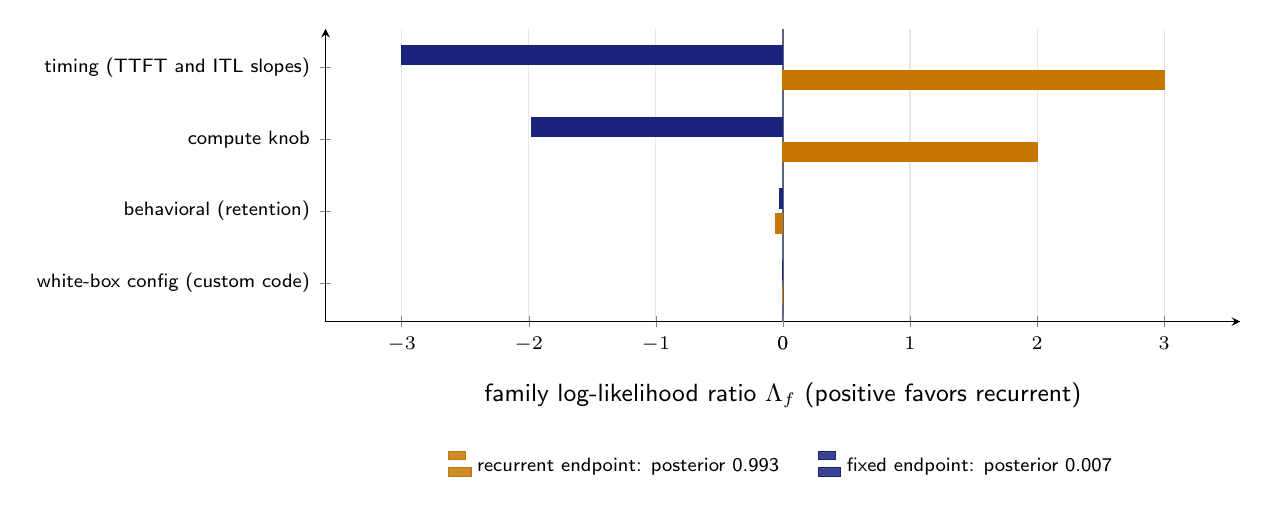
\begin{tikzpicture}
\begin{axis}[
  xbar, width=13.2cm, height=5.3cm,
  xmin=-3.6, xmax=3.6,
  bar width=7pt,
  symbolic y coords={config,behavioral,knob,timing},
  ytick={config,behavioral,knob,timing},
  yticklabels={white-box config (custom code), behavioral (retention), compute knob, timing (TTFT and ITL slopes)},
  y tick label style={font=\sffamily\scriptsize, align=right},
  tick label style={font=\sffamily\scriptsize},
  xlabel={family log-likelihood ratio $\Lambda_f$ (positive favors recurrent)},
  label style={font=\sffamily\small},
  axis lines=left, xmajorgrids, grid style={medgray!40},
  enlarge y limits=0.18,
  legend style={font=\sffamily\scriptsize, draw=none, fill=white, fill opacity=0.85, text opacity=1, at={(0.5,-0.42)}, anchor=north, legend columns=2, /tikz/every even column/.append style={column sep=1.2em}},
  extra x ticks={0}, extra x tick style={grid style={softslate, line width=0.8pt}},
]
\addplot[fill=darkamber, draw=darkamber] coordinates {(3.0,timing) (2.0,knob) (-0.06,behavioral) (0.0,config)};
\addlegendentry{recurrent endpoint: posterior 0.993}
\addplot[fill=deepindigo, draw=deepindigo] coordinates {(-3.0,timing) (-1.98,knob) (-0.03,behavioral) (0.0,config)};
\addlegendentry{fixed endpoint: posterior 0.007}
\end{axis}
\end{tikzpicture}
\caption[Family contributions in the synthetic worked example]{Two independent families agreeing is what decides a verdict. Family contributions in the synthetic worked example, with likelihoods fitted to a simulated reference fleet and a prior of 0.5: timing and the compute knob agree in each case, so both verdicts are decided, while the behavioral family contributes almost nothing.}
\label{fig:waterfall}
\end{figure}

% ============================================================================
% PART III
% ============================================================================
\partbanner{III}{Validation and Practice}{Benchmarking on known models, the toolkit, guardrails, recommendations, and checklists}{%
  % a calibration curve with reference points
  \draw[white, opacity=0.35, line width=0.6pt] (0.4,0.9) -- (0.4,6.6);
  \draw[white, opacity=0.35, line width=0.6pt] (0.4,0.9) -- (7.8,0.9);
  \draw[white, opacity=0.25, dashed, line width=0.6pt] (0.4,0.9) -- (7.6,6.4);
  \draw[honeyamber, line width=1.6pt] plot[domain=0:1, samples=40, smooth] ({0.4+7.2*\x},{0.9+5.5*(\x^1.6/(\x^1.6+(1-\x)^1.6))});
  \foreach \x/\y in {1.0/1.1, 1.6/1.3, 2.3/1.8, 5.6/5.0, 6.4/5.9, 7.1/6.2} {
    \fill[white, opacity=0.85] (\x,\y) circle (0.09);
  }
  \foreach \x/\y in {3.4/3.0, 4.2/3.9} {
    \draw[honeyamber, line width=0.9pt] (\x,\y) circle (0.12);
  }
}

% ============================================================================
% SECTION 7: VALIDATION
% ============================================================================
\section{Validation on Known Models}
\label{sec:validation}

\inbrief{Before measuring an undisclosed model, measure models whose architecture is documented, with the same plan and serving setup, and report the classifier's coverage and errors under leave-one-out.}

\subsection{Reference Sets}

{\small
\zebra
\begin{tabularx}{\textwidth}{L{4.4cm} Y}
\rowcolor{deepindigo}
\hd{Group} & \hd{Candidates (open weights)} \\
Looped, sampled count & Huginn-0125~[4] \\
Looped, fixed count with exit gate & Ouro-1.4B, Ouro-2.6B and Thinking variants~[5] \\
Looped, fixed count & Nanbeige4.2-3B~[59]; Nemotron Labs Dory 1.0 4B at a set loop count~[66] \\
Retrofitted recurrence & Released retrofitting checkpoints~[8] \\
Token-level recursion & Mixture-of-Recursions checkpoints, where released~[6] \\
Fixed depth, similar size & Qwen2.5 0.5B to 3B, SmolLM2, OLMo-2, Llama 3.2 \\
Confounder controls & An MoE model (Qwen1.5-MoE-A2.7B); an early-exit model (LayerSkip checkpoints~[16]); a speculative-decoding server configuration \\
\tablefinish
\end{tabularx}\par}
\medskip

Serve all of them with the same inference server, hardware, batching settings, and sampling parameters. A difference in serving stack can produce a timing difference larger than the architectural one.

\subsection{Protocol}

\begin{figure}[htbp]
\centering
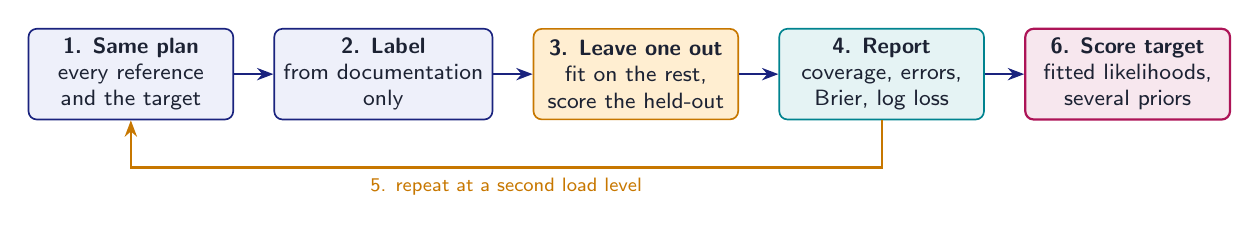
\begin{tikzpicture}[font=\sffamily\footnotesize, node distance=0.5cm]
  \node[flowstep, minimum width=2.6cm, minimum height=1.15cm] (s1) {\textbf{1. Same plan}\\every reference\\and the target};
  \node[flowstep, minimum width=2.6cm, minimum height=1.15cm, right=of s1] (s2) {\textbf{2. Label}\\from documentation\\only};
  \node[loopbox, minimum width=2.6cm, minimum height=1.15cm, right=of s2] (s3) {\textbf{3. Leave one out}\\fit on the rest,\\score the held-out};
  \node[observe, minimum width=2.6cm, minimum height=1.15cm, right=of s3] (s4) {\textbf{4. Report}\\coverage, errors,\\Brier, log loss};
  \node[hot, minimum width=2.6cm, minimum height=1.15cm, right=of s4] (s5) {\textbf{6. Score target}\\fitted likelihoods,\\several priors};
  \draw[arr] (s1) -- (s2);
  \draw[arr] (s2) -- (s3);
  \draw[arr] (s3) -- (s4);
  \draw[arr] (s4) -- (s5);
  \draw[aarr] (s4.south) -- ++(0,-0.6) -| node[pos=0.25, below, font=\sffamily\scriptsize, text=darkamber] {5. repeat at a second load level} (s1.south);
\end{tikzpicture}
\caption[Validation protocol]{Validation protocol. The target is scored only after the classifier's error rate on documented models is known.}
\label{fig:protocol}
\end{figure}

\begin{enumerate}
  \item Run the identical probe plan against every reference and the target.
  \item Label references from their documentation only.
  \item Leave each reference out in turn, fit likelihoods to the rest, and score it.
  \item Report coverage (fraction decided), accuracy among decided verdicts, the number of wrong decided verdicts, Brier score, and log loss.
  \item Repeat at more than one load level (quiet and busy hours), because batching changes timing.
  \item Only then score the target, with the fitted likelihoods and several priors.
\end{enumerate}

\subsection{Results So Far}
\label{sec:results}

{\footnotesize
\zebra
\begin{tabularx}{\textwidth}{L{3.3cm} L{3.4cm} Y}
\rowcolor{deepindigo}
\hd{Check} & \hd{Data} & \hd{Result} \\
Config inspection & 8 published configs & All correct: Huginn-0125, Ouro-1.4B, Ouro-2.6B-Thinking, ALBERT-base-v2 recurrent or weight-shared; Qwen2.5-0.5B, SmolLM2-135M, OLMo-2-1B standard; Qwen1.5-MoE-A2.7B standard with an MoE note \\
Weight sharing, real fixed model & SmolLM2-135M (30 layers) & 30 distinct layers, no exact or low-rank pairs, adjacent distance 1.32 to 1.41 (no false positive) \\
Dynamics, real fixed model & SmolLM2-135M, 48 tokens & Tail contraction 1.12 (not converging), periodicity excess 0.002 \\
Scoring, synthetic fleet & 6 fixed and 6 recurrent simulated endpoints & Leave-one-out coverage 0.67, 0 wrong decided verdicts, Brier 0.016; of the 4 undecided, 3 were recurrent and 1 fixed \\
Black-box probes, real APIs & none yet & \textbf{Not yet run} \\
\tablefinish
\end{tabularx}\par}

\begin{warnbox}[What has not been done]
No black-box measurement of any real endpoint has been made for this guide, and the white-box checks have not yet been run on a real looped model's weights or per-iteration activations. The simulated fleet tests the pipeline, not the world. The first real benchmark should be the reference set above.
\end{warnbox}

\subsection{Adversarial Robustness}

A provider that does not want its architecture inferred can pad latency to a constant per token or buffer tokens and release them at fixed intervals, both of which Majidi et al. discuss as defenses at a cost in latency~[32]. Either would remove the timing family. Behavioral and compute-knob signals would remain, but they are the weaker ones. \mE\ External detection is therefore a complement to disclosure, not a substitute for it.

% ============================================================================
% SECTION 8: TOOLKIT
% ============================================================================
\section{The Toolkit}
\label{sec:toolkit}

\inbrief{One command per measurement, all printing JSON signal files that \cfg{score} combines. The package README has a quickstart that runs end to end, from a local checkpoint and a simulated endpoint to a validated, scored verdict.}

The companion package \texttt{packages/recurrent\_depth/} implements the measurements and scoring above. It depends only on numpy (torch and transformers are needed only for \cfg{capture-hidden}), runs in the repository's \texttt{python-ci} container, and its tests run without network or GPU. Nothing in it downloads a model.

{\footnotesize
\zebra
\begin{tabularx}{\textwidth}{L{3.5cm} L{1.6cm} Y}
\rowcolor{deepindigo}
\hd{Command} & \hd{Section} & \hd{What it does} \\
\cfg{inspect-config} & \ref{sec:config} & Classifies a \cfg{config.json}; reports declared loops, exit settings, MoE fields, stored versus logical depth \\
\cfg{inspect-weights} & \ref{sec:sharing} & Memory-maps safetensors (including sharded, BF16, and FP8), finds exact and low-rank layer sharing and missing layer indices, compares declared and stored depth \\
\cfg{capture-hidden} & \ref{sec:converge} & Records per-layer hidden states and the unembedding from a local Hugging Face checkpoint; a looped model's per-iteration states may need hooks in its own code \\
\cfg{analyze-hidden} & \ref{sec:similarity}--\ref{sec:converge} & Contraction, similarity periodicity, and logit-lens settling steps from a recorded trajectory \\
\cfg{probe} & \ref{sec:blackbox} & Runs a seeded, interleaved serial-depth plan against an OpenAI-compatible endpoint with a hard request budget (retries included), rate limit, backoff, a terms acknowledgement, and no redirects (so a key is never forwarded) \\
\cfg{features} & \ref{sec:blackbox} & Computes timing slopes, serial retention, and knob effects; drops requests with hidden reasoning tokens and reports the TTFT effect in inter-token latencies \\
\cfg{score} & \ref{sec:scoring} & Combines signal files into a verdict with per-family contributions and notes \\
\cfg{fit}, \cfg{validate} & \ref{sec:validation} & Fits likelihoods to labeled references; leave-one-out benchmark \\
\cfg{simulate}, \cfg{simulate-fleet} & \ref{sec:worked} & Synthetic endpoints for offline testing \\
\tablefinish
\end{tabularx}\par}

\textbf{A first run.} The sequence below is the README quickstart with file paths shortened. Step~4 reproduces the worked example of Section~\ref{sec:worked} (posterior 0.993, \textbf{recurrent}); step~3 reproduces the synthetic-fleet row of Section~\ref{sec:results}. For a real endpoint, replace \cfg{simulate} with \cfg{probe plan.json -{}-out records.jsonl} after setting \cfg{acknowledge\_terms} truthfully, and measure the reference models with the same plan first.

\begin{codebox}
\begin{verbatim}
rd() { docker compose --profile ci run --rm -T \
         -e PYTHONPATH=packages/recurrent_depth/src python-ci \
         python -m recurrent_depth "$@"; }

# 1. White box: a local checkpoint in $M (nothing is downloaded)
rd inspect-config  $M/config.json             > config.json
rd inspect-weights $M --config $M/config.json > weights.json
rd capture-hidden  $M --text "..." --out states.npy --unembed-out unembed.npy
rd analyze-hidden  states.npy --unembed unembed.npy > dynamics.json

# 2. Black box: a simulated adaptive recurrent endpoint
rd simulate --kind recurrent --knob --out rec.jsonl
rd features rec.jsonl --knob-order low,medium,high > rec_signals.json

# 3. Calibrate and validate on labeled references
rd simulate-fleet --n-each 6 --out refs.json
rd validate refs.json
rd fit refs.json --out models.json

# 4. Score (config unknown, as for custom code)
echo '{"signals": {"config_recurrence": 0.5}}' > custom_code.json
rd score rec_signals.json custom_code.json --models models.json
\end{verbatim}
\end{codebox}

On SmolLM2-135M, scoring \cfg{config.json} and \cfg{weights.json} from step~1 returns \textbf{inconclusive} (posterior 0.10), as intended: a standard config and unshared weights are absences, and absences never decide alone.

% ============================================================================
% SECTION 9: GUARDRAILS
% ============================================================================
\section{Guardrails and Responsible Disclosure}
\label{sec:guardrails}

\inbrief{Measure, do not extract. Stay inside the provider's terms and the law. Tell the provider before you tell the world.}

\begin{itemize}
  \item \textbf{Terms and law.} Query only endpoints you are authorized to use, within their terms of service and rate limits. Take legal advice where terms are unclear; this guide is not legal advice.
  \item \textbf{No extraction.} Do not attempt to recover weights, embedding matrices, or training data. Width estimation is limited to vectors you are entitled to collect, at your normal rate limits, and is reported as a single number.
  \item \textbf{No access-control bypass.} Do not use multiple accounts to evade rate limits, spoof clients, or probe infrastructure other than the public API.
  \item \textbf{No harm to other users.} Do not use techniques that infer other customers' prompts or traffic. Several published timing attacks do exactly that~[33,34]; they are cited here as confounders, not methods.
  \item \textbf{Disclose first.} Share findings that reveal a provider's undisclosed design with the provider before publishing, and give them time to respond, as Majidi et al. did by disclosing their speculative-decoding attack to the affected provider months before publication~[32].
  \item \textbf{Publish carefully.} Publish verdicts with their evidence, priors, coverage, and error rates. Never publish a verdict without its uncertainty, and never present a reported architecture as fact.
\end{itemize}

% ============================================================================
% SECTION 10: RECOMMENDATIONS
% ============================================================================
\section{Recommendations}
\label{sec:recs}

\subsection{For Evaluators}
\begin{enumerate}
  \item Measure single-pass serial capability (no-CoT accuracy against controlled depth) for every frontier model you evaluate, whatever its architecture.
  \item Ask developers for architecture details under your access agreement before inferring them.
  \item When you infer, publish the method, the reference benchmark, and the inconclusive rate.
\end{enumerate}

\subsection{For Developers}
\label{sec:recdev}
\begin{enumerate}
  \item Disclose loop counts, whether they are adaptive, and their range at inference, in model or system cards.
  \item Report chain-of-thought monitorability and no-CoT capability together, as the Astra card does~[50], and say whether in-pass recurrence contributes. Without that statement, readers cannot tell an architecture-driven decline from a capability-driven one (Section~\ref{sec:astra}).
  \item Offer per-iteration readouts (decoded intermediate states) to monitors and auditors, since looped models can produce them~[5].
  \item Count training and inference compute directly, not from parameter counts.
\end{enumerate}

\subsection{For Policy Bodies}
\begin{enumerate}
  \item Require disclosure of maximum serial depth per token (layers times loops) alongside parameter count for models above existing compute thresholds.
  \item Do not estimate compute from parameter counts for models that may reuse parameters.
  \item Treat external architecture inference as evidence that prompts questions, not as findings, unless it is benchmarked and decisive.
\end{enumerate}

\subsection{For Deployers: Architecture-Aware Model Selection}
\label{sec:recdeploy}

Organizations that run frontier models in agentic or tool-using settings inherit the developer's ability to verify alignment. When a developer reports that reasoning-based monitoring has become less reliable, or a model is credibly reported to move reasoning out of the trace, a written policy is better than case-by-case vendor decisions. One reasonable pattern, offered as an example rather than an endorsement of any vendor or model:

\begin{enumerate}
  \item \textbf{A criterion keyed to architecture and reported monitorability, not to a vendor.} Exclude from sensitive environments (production, and lower environments that share credentials, code, or network paths with it) any model whose developer documents it as relying substantially on in-pass recurrence, or reports that CoT-based monitoring is unreliable against it. The rule applies to every vendor equally, including incumbents.\\
  \emph{Tradeoff:} it depends on disclosures that may be absent; external detection (Sections~\ref{sec:methods}--\ref{sec:validation}) can raise questions but rarely settles them; it may exclude the most capable model.
  \item \textbf{An evaluation-only exception.} Excluded models may run in isolated environments with no organizational data, credentials, or network reach beyond the evaluation harness, with named approval and full logging.\\
  \emph{Tradeoff:} isolation costs effort, but it builds the comparative evidence the policy needs.
  \item \textbf{Revisit triggers}, each with an owner and a review date, or the policy goes stale. Reconsider when:
  \begin{itemize}
    \item the developer publishes per-release loop-count and monitorability metrics;
    \item third-party stealth and sabotage evaluations reach parity with those for conventional models;
    \item verification methods that do not depend on legible CoT are externally validated;
    \item the architecture becomes universal, so exclusion is no longer available and the policy must become a control-based posture.
  \end{itemize}
\end{enumerate}

\begin{keybox}[Controls needed regardless of the model]
None of these depends on reading the model's reasoning, so they keep their value whatever the architecture:
\begin{itemize}
  \item policy checks on outputs and tool calls before execution;
  \item least-privilege, per-task tool permissions without ambient credentials;
  \item sandboxed execution with egress control;
  \item behavioral evaluations on the organization's own workloads, including sabotage and impossible-task scenarios;
  \item a model abstraction layer, so that switching providers is a configuration change;
  \item tool-call and output logs kept independently of vendor retention.
\end{itemize}
\end{keybox}

\mE\ Two cautions. First, because behavioral metrics cannot separate architecture from capability (Section~\ref{sec:astra}), a criterion keyed only to architecture can miss a model whose monitorability fell for other reasons; keying on reported monitorability as well closes that gap. Second, a criterion keyed on what developers report penalizes the developers who measure and report most. A policy should say so, and treat a developer's measurement and disclosure practice as evidence in its favor rather than against it.

\subsection{Open Research Problems}
\begin{itemize}
  \item Extending per-token timing models~[32] to looped and MoE architectures.
  \item Testing whether intermediate loop readouts are faithful enough to monitor.
  \item Measuring whether looped models vary hidden effort on evaluation-like inputs.
  \item Validating the manipulation-versus-storage contrast as a black-box classifier.
\end{itemize}

% ============================================================================
% SECTION 11: CHECKLISTS
% ============================================================================
\section{Checklists}
\label{sec:checklists}

\begin{tcbraster}[raster columns=3, raster equal height, raster column skip=8pt]
\begin{tcolorbox}[checkcard, title={\ding{110}\hspace{0.4em}Before probing}]
\begin{checklist}
  \item Authorized to use the endpoint; plan within terms and rate limits
  \item Budget and rate limit set; \cfg{acknowledge\_terms} set truthfully
  \item Reference models chosen and served on the same stack
  \item Classifier benchmarked leave-one-out on the references
  \item Priors written down before seeing target results
\end{checklist}
\end{tcolorbox}
\begin{tcolorbox}[checkcard, colframe=darkamber, colbacktitle=darkamber, title={\ding{110}\hspace{0.4em}Per measurement run}]
\begin{checklist}
  \item Prompt length constant across depths in each family
  \item Output capped and constant; temperature 0
  \item Conditions interleaved in a seeded random order
  \item Requests with hidden reasoning tokens excluded
  \item Run repeated at a second load level
\end{checklist}
\end{tcolorbox}
\begin{tcolorbox}[checkcard, colframe=campaignred, colbacktitle=campaignred, title={\ding{110}\hspace{0.4em}Before publishing}]
\begin{checklist}
  \item Posterior, family contributions, and priors reported
  \item Coverage and errors from validation reported
  \item Confounders not excluded are listed
  \item Provider informed and given time to respond
  \item Reported or rumored claims labeled as such
\end{checklist}
\end{tcolorbox}
\end{tcbraster}

% ============================================================================
% SECTION 12: REFERENCES
% ============================================================================
\section{References}
\label{sec:refs}

\begingroup
\small
\sloppy
\setstretch{1.05}
\begin{enumerate}[label={\textcolor{deepindigo}{[\arabic*]}}, leftmargin=2.6em, itemsep=0.3em]
  \item M.~Dehghani et al., \emph{Universal Transformers}, arXiv:1807.03819, ICLR 2019. \url{https://arxiv.org/abs/1807.03819}
  \item A.~Graves, \emph{Adaptive Computation Time for Recurrent Neural Networks}, arXiv:1603.08983, 2016. \url{https://arxiv.org/abs/1603.08983}
  \item A.~Banino, J.~Balaguer, and C.~Blundell, \emph{PonderNet: Learning to Ponder}, arXiv:2107.05407, 2021. \url{https://arxiv.org/abs/2107.05407}
  \item J.~Geiping et al., \emph{Scaling up Test-Time Compute with Latent Reasoning: A Recurrent Depth Approach}, arXiv:2502.05171, 2025; weights released as \texttt{tomg-group-umd/huginn-0125}. \url{https://arxiv.org/abs/2502.05171}
  \item R.-J.~Zhu et al., \emph{Scaling Latent Reasoning via Looped Language Models} (Ouro), arXiv:2510.25741, October 2025 (revised October 2026). \url{https://arxiv.org/abs/2510.25741}
  \item S.~Bae et al., \emph{Mixture-of-Recursions: Learning Dynamic Recursive Depths for Adaptive Token-Level Computation}, arXiv:2507.10524, 2025. \url{https://arxiv.org/abs/2507.10524}
  \item S.~Bae et al., \emph{Relaxed Recursive Transformers: Effective Parameter Sharing with Layer-wise LoRA}, arXiv:2410.20672, ICLR 2025. \url{https://arxiv.org/abs/2410.20672}
  \item S.~McLeish et al., \emph{Teaching Pretrained Language Models to Think Deeper with Retrofitted Recurrence}, arXiv:2511.07384, 2025. \url{https://arxiv.org/abs/2511.07384}
  \item M.~Shapiro, \emph{Retrofitting Recurrent Depth into a Pretrained Language Model: Installation, Extrapolation, Transfer, and Retention at Two Parameter Budgets}, arXiv:2608.11233, 2026. \url{https://arxiv.org/abs/2608.11233}
  \item S.~Hao et al., \emph{Training Large Language Models to Reason in a Continuous Latent Space} (Coconut), arXiv:2412.06769, COLM 2025. \url{https://arxiv.org/abs/2412.06769}
  \item S.~Goyal et al., \emph{Think before you speak: Training Language Models With Pause Tokens}, arXiv:2310.02226, ICLR 2024. \url{https://arxiv.org/abs/2310.02226}
  \item J.~Pfau, W.~Merrill, and S.~R.~Bowman, \emph{Let's Think Dot by Dot: Hidden Computation in Transformer Language Models}, arXiv:2404.15758, 2024. \url{https://arxiv.org/abs/2404.15758}
  \item G.~Wang et al., \emph{Hierarchical Reasoning Model}, arXiv:2506.21734, 2025. \url{https://arxiv.org/abs/2506.21734}
  \item A.~Jolicoeur-Martineau, \emph{Less is More: Recursive Reasoning with Tiny Networks}, arXiv:2510.04871, 2025. \url{https://arxiv.org/abs/2510.04871}
  \item T.~Schuster et al., \emph{Confident Adaptive Language Modeling}, arXiv:2207.07061, NeurIPS 2022. \url{https://arxiv.org/abs/2207.07061}
  \item M.~Elhoushi et al., \emph{LayerSkip: Enabling Early Exit Inference and Self-Speculative Decoding}, arXiv:2404.16710, ACL 2024. \url{https://arxiv.org/abs/2404.16710}
  \item D.~Raposo et al., \emph{Mixture-of-Depths: Dynamically allocating compute in transformer-based language models}, arXiv:2404.02258, 2024. \url{https://arxiv.org/abs/2404.02258}
  \item Y.~Leviathan, M.~Kalman, and Y.~Matias, \emph{Fast Inference from Transformers via Speculative Decoding}, arXiv:2211.17192, ICML 2023. \url{https://arxiv.org/abs/2211.17192}
  \item N.~Saunshi, N.~Dikkala, Z.~Li, S.~Kumar, and S.~J.~Reddi, \emph{Reasoning with Latent Thoughts: On the Power of Looped Transformers}, arXiv:2502.17416, ICLR 2025. \url{https://arxiv.org/abs/2502.17416}
  \item A.~Giannou, S.~Rajput, J.~Sohn, K.~Lee, J.~D.~Lee, and D.~Papailiopoulos, \emph{Looped Transformers as Programmable Computers}, arXiv:2301.13196, 2023. \url{https://arxiv.org/abs/2301.13196}
  \item L.~Yang, K.~Lee, R.~Nowak, and D.~Papailiopoulos, \emph{Looped Transformers are Better at Learning Learning Algorithms}, arXiv:2311.12424, ICLR 2024. \url{https://arxiv.org/abs/2311.12424}
  \item Y.~Fan, Y.~Du, K.~Ramchandran, and K.~Lee, \emph{Looped Transformers for Length Generalization}, arXiv:2409.15647, ICLR 2025. \url{https://arxiv.org/abs/2409.15647}
  \item W.~Merrill and A.~Sabharwal, \emph{The Expressive Power of Transformers with Chain of Thought}, arXiv:2310.07923, ICLR 2024. \url{https://arxiv.org/abs/2310.07923}
  \item W.~Merrill and A.~Sabharwal, \emph{A Little Depth Goes a Long Way: The Expressive Power of Log-Depth Transformers}, arXiv:2503.03961, NeurIPS 2025. \url{https://arxiv.org/abs/2503.03961}
  \item W.~Merrill, J.~Petty, and A.~Sabharwal, \emph{The Illusion of State in State-Space Models}, arXiv:2404.08819, ICML 2024. \url{https://arxiv.org/abs/2404.08819}
  \item M.~Hahn, \emph{Theoretical Limitations of Self-Attention in Neural Sequence Models}, arXiv:1906.06755, TACL 2020. \url{https://arxiv.org/abs/1906.06755}
  \item T.~Korbak et al., \emph{Chain of Thought Monitorability: A New and Fragile Opportunity for AI Safety}, arXiv:2507.11473, 2025. \url{https://arxiv.org/abs/2507.11473}
  \item B.~Baker et al., \emph{Monitoring Reasoning Models for Misbehavior and the Risks of Promoting Obfuscation}, arXiv:2503.11926, 2025. \url{https://arxiv.org/abs/2503.11926}
  \item S.~Emmons et al., \emph{When Chain of Thought is Necessary, Language Models Struggle to Evade Monitors}, arXiv:2507.05246, 2025. \url{https://arxiv.org/abs/2507.05246}
  \item N.~Carlini et al., \emph{Stealing Part of a Production Language Model}, arXiv:2403.06634, ICML 2024. \url{https://arxiv.org/abs/2403.06634}
  \item M.~Finlayson, X.~Ren, and S.~Swayamdipta, \emph{Logits of API-Protected LLMs Leak Proprietary Information}, arXiv:2403.09539, COLM 2024. \url{https://arxiv.org/abs/2403.09539}
  \item S.~Majidi, N.~Mireshghallah, and K.~Taram, \emph{Leaky Language Models: Stealing Architecture and Inference Optimizations via Per-Token Timing}, arXiv:2607.20723, July 2026. \url{https://arxiv.org/abs/2607.20723}
  \item N.~Carlini and M.~Nasr, \emph{Remote Timing Attacks on Efficient Language Model Inference}, arXiv:2410.17175, 2024. \url{https://arxiv.org/abs/2410.17175}
  \item T.~Zhang, G.~Saileshwar, and D.~Lie, \emph{Time Will Tell: Timing Side Channels via Output Token Count in Large Language Models}, arXiv:2412.15431, 2024. \url{https://arxiv.org/abs/2412.15431}
  \item D.~Pasquini, E.~M.~Kornaropoulos, and G.~Ateniese, \emph{LLMmap: Fingerprinting For Large Language Models}, arXiv:2407.15847, USENIX Security 2025. \url{https://arxiv.org/abs/2407.15847}
  \item M.~Sun et al., \emph{Idiosyncrasies in Large Language Models}, arXiv:2502.12150, ICML 2025. \url{https://arxiv.org/abs/2502.12150}
  \item nostalgebraist, \emph{interpreting GPT: the logit lens}, LessWrong, 31 August 2020. \url{https://www.lesswrong.com/posts/AcKRB8wDpdaN6v6ru/interpreting-gpt-the-logit-lens}
  \item N.~Belrose et al., \emph{Eliciting Latent Predictions from Transformers with the Tuned Lens}, arXiv:2303.08112, 2023. \url{https://arxiv.org/abs/2303.08112}
  \item S.~Kornblith, M.~Norouzi, H.~Lee, and G.~Hinton, \emph{Similarity of Neural Network Representations Revisited}, arXiv:1905.00414, ICML 2019. \url{https://arxiv.org/abs/1905.00414}
  \item W.~Lu, Y.~Yang, K.~Lee, Y.~Li, and E.~Liu, \emph{Latent Chain-of-Thought? Decoding the Depth-Recurrent Transformer}, arXiv:2507.02199, 2025 (COLM 2025 workshop). \url{https://arxiv.org/abs/2507.02199}
  \item S.~Bai, J.~Z.~Kolter, and V.~Koltun, \emph{Deep Equilibrium Models}, arXiv:1909.01377, NeurIPS 2019. \url{https://arxiv.org/abs/1909.01377}
  \item K.~Schwethelm, D.~Rueckert, and G.~Kaissis, \emph{Depth-adaptive Inference of Looped Language Models via Continuous Depth Batching}, arXiv:2608.09444, 2026. \url{https://arxiv.org/abs/2608.09444}
  \item R.~Lin, Y.~Guo, R.-J.~Zhu, H.~Ye, and J.~K.~Eshraghian, \emph{Allocating Recurrent Compute in Looped Language Models}, arXiv:2608.18230, 2026. \url{https://arxiv.org/abs/2608.18230}
  \item A.~Jeddi, M.~Ciccone, and B.~Taati, \emph{LoopFormer: Elastic-Depth Looped Transformers for Latent Reasoning via Shortcut Modulation}, arXiv:2602.11451, ICLR 2026. \url{https://arxiv.org/abs/2602.11451}
  \item Y.~Wang et al., \emph{RecurTrace: Adaptive Latent Reasoning with Loop-Time Memory}, arXiv:2609.03379, 2026. \url{https://arxiv.org/abs/2609.03379}
  \item J.~Fein-Ashley and P.~Rashidinejad, \emph{Solve the Loop: Attractor Models for Language and Reasoning}, arXiv:2605.12466, 2026. \url{https://arxiv.org/abs/2605.12466}
  \item A.~Gromov et al., \emph{The Unreasonable Ineffectiveness of the Deeper Layers}, arXiv:2403.17887, ICLR 2025. \url{https://arxiv.org/abs/2403.17887}
  \item V.~Lad et al., \emph{The Remarkable Robustness of LLMs: Stages of Inference?}, arXiv:2406.19384, 2024. \url{https://arxiv.org/abs/2406.19384}
  \item S.~Yang et al., \emph{Do Large Language Models Latently Perform Multi-Hop Reasoning?}, arXiv:2402.16837, ACL 2024. \url{https://arxiv.org/abs/2402.16837}
  \item OpenAI, \emph{GPT-6 Astra System Card}, Deployment Safety Hub, September 2026. \url{https://deploymentsafety.openai.com/gpt-6-astra}
  \item J.~Kahn, \emph{Safety experts warn novel design of OpenAI's Astra model could make future AI agents harder to monitor}, Fortune, 3 September 2026. \url{https://fortune.com/2026/09/03/reports-openais-astra-model-uses-a-new-more-efficient-ai-architecture-alarms-ai-safety-experts-who-worry-the-method-makes-models-harder-to-control/}
  \item J.~Pachocki, post on X, 2 September 2026. \url{https://x.com/merettm/status/2095023204993490967}
  \item S.~Raschka, \emph{GPT-6 Astra, Looped Transformers, and Hidden Reasoning}, 9 September 2026. \url{https://magazine.sebastianraschka.com/p/gpt-6-astra-looped-transformers-and}
  \item R.~Arike, \emph{How concerned should we be about Astra's recurrent architecture?}, LessWrong, 2 September 2026. \url{https://www.lesswrong.com/posts/PLisnSFir8y5AHkmP/how-concerned-should-we-be-about-astra-s-recurrent}
  \item A.~Efrati, \emph{Exclusive: OpenAI Technique in `Astra' Model Sparks Security Concerns}, The Information, 1 September 2026 (paywalled; not read directly for this guide; known through [51], [53], and [58]). \url{https://www.theinformation.com/articles/secret-technique-behind-openais-astra-model-sparks-security-concerns}
  \item European Union, \emph{Artificial Intelligence Act}, Article 51 (classification of general-purpose AI models with systemic risk). \url{https://artificialintelligenceact.eu/article/51/}
  \item F.~Gloeckle, B.~Youbi Idrissi, B.~Rozi\`ere, D.~Lopez-Paz, and G.~Synnaeve, \emph{Better \& Faster Large Language Models via Multi-token Prediction}, arXiv:2404.19737, ICML 2024. \url{https://arxiv.org/abs/2404.19737}
  \item R.~Brandom, \emph{OpenAI's new reasoning technique alarms AI safety experts}, TechCrunch, 2 September 2026. \url{https://techcrunch.com/2026/09/02/openais-new-reasoning-technique-alarms-ai-safety-experts/}
  \item Nanbeige LLM Lab, \emph{Nanbeige4.2-3B} model card and config, Hugging Face, July 2026 (technical report arXiv:2607.22083). \url{https://huggingface.co/Nanbeige/Nanbeige4.2-3B}
  \item J.~Pachocki, \emph{An Alien Mind}, OpenAI, 6 September 2026 (page not retrievable for this review; quoted as reproduced in press coverage). \url{https://openai.com/index/an-alien-mind/}
  \item AFP, \emph{OpenAI shelves new AI model release over safety concerns}, via Cyprus Mail, 29 September 2026. \url{https://cyprus-mail.com/2026/09/29/openai-shelves-new-ai-model-release-over-safety-concerns}
  \item TechCrunch, \emph{OpenAI cuts ties with 3 safety researchers, WSJ reports}, 1 October 2026. \url{https://techcrunch.com/2026/10/01/openai-cuts-ties-with-three-safety-researchers-wsj-reports/}
  \item K.~Chan, \emph{OpenAI fires 3 safety researchers in dispute over AI risks}, Associated Press, 9 October 2026 (via News4JAX). \url{https://www.news4jax.com/business/2026/10/09/openai-fires-3-safety-researchers-in-dispute-over-ai-risks/}
  \item B.~Fisher, \emph{OpenAI Fired Three Researchers Who Said Loop Transformer Would Blind Safety Monitors}, Tech Times, 15 October 2026 (secondary coverage of a paywalled report in The Information, 13 October 2026). \url{https://www.techtimes.com/articles/329046/20261014/openai-fired-three-researchers-who-said-loop-transformer-would-blind-safety-monitors.htm}
  \item Anthropic, \emph{Claude Opus 5.5 System Card}, 22 September 2026, sections 6.6.1 and 6.6.4. \url{https://www.anthropic.com/document/claude-opus-5-5-system-card}
  \item NVIDIA, \emph{NVIDIA Nemotron Labs Dory 1.0 4B} model card, Hugging Face, 16 October 2026. \url{https://huggingface.co/nvidia/NVIDIA-Nemotron-Labs-Dory1.0-4B-BF16}
\end{enumerate}
\endgroup

% ============================================================================
% DOCUMENT HISTORY
% ============================================================================
\vspace{1.2em}
\phantomsection
\subsection*{Document History}
\addcontentsline{toc}{section}{Document History}
\markboth{Document History}{}

{\small
\zebra
\begin{tabularx}{\textwidth}{L{1.4cm} L{2.4cm} Y}
\rowcolor{deepindigo}
\hd{Version} & \hd{Date} & \hd{Changes} \\
1.0 & October 2026 & Initial release, with companion toolkit \texttt{packages/recurrent\_depth}. Before release (late October 2026) the guide and toolkit were verified and reviewed. \textbf{Corrections:} Fortune headline and author [51]; ``OpenAI did not deny'' replaced by Fortune's own wording; Pachocki's post quoted in full; The Information headline and author [55]; Huginn saturation stated as 8 to 12 iterations; continuous depth batching's 99\% figure tied to Ouro [42]; speculative-decoding timing described as draft-target agreement [32]; the unused reference [43] now cited; author names and venues completed; the Associated Press article [63] given its headline, author, and date (9 October 2026), and OpenAI's statement on the researcher dismissals quoted as that article reports it; the Opus 5.5 card's controllability points and internal-use sample described as the card states them. \textbf{Reader experience:} executive summary rewritten to carry the whole argument; a detection-methods-at-a-glance figure (Figure~\ref{fig:glance}) replaces the evidence ladder; takeaway captions; the deployer table restructured as a list; a first-run command sequence in Section~\ref{sec:toolkit}. \textbf{Additions:} verified Astra system-card measurements and the Opus 5.5 card's separate measurements (Section~\ref{sec:astra}, Figure~\ref{fig:astracard}), the September--October timeline (GPT-6.1 Astra delay, researcher dismissals, reporting on OpenAI's next model), the argument that behavioral metrics cannot separate architecture from capability (Figure~\ref{fig:attribution}), Nanbeige4.2-3B and NVIDIA's Nemotron Labs Dory 1.0 4B (released 16 October 2026) [66], more timing confounders (multi-token prediction, rate limiting, gateway buffering, quantization, connection setup, unreported hidden tokens), notes on the scorer's correlation heuristic, and Section~\ref{sec:recdeploy} for deployers. \textbf{Toolkit fixes:} monotone likelihood ratios (a negative latency slope no longer counts toward recurrence); one-sided weight signals and a white-box decision threshold of 3 (unshared weights in Ouro-style checkpoints no longer decide ``fixed''); single-group (ALBERT-style) and gapped layer stacks; FP8 and endian-safe safetensors reads with offset checks; redirects refused so keys are never forwarded; hard request budget including retries; mid-stream errors recorded; knob accuracy gain computed without hidden-token requests; a reachability generator hang removed; unsettled tokens distinguished in logit-lens settling; a \cfg{capture-hidden} command, option help, and an end-to-end README quickstart. Synthetic worked-example and fleet numbers recomputed (Sections~\ref{sec:worked} and \ref{sec:results}) \\
\tablefinish
\end{tabularx}\par}

\vspace{1em}
{\small\color{softslate}\emph{Independent research, not affiliated with any institution or committee. Published for AI safety research, evaluation, and education. MIT License.}\par}

\end{document}
